\documentclass[aspectratio=169,9pt]{beamer}
\usepackage{amsmath,amssymb}
\usepackage{graphicx}
\usepackage{booktabs}

\usetheme{default}
\setbeamertemplate{navigation symbols}{}
\setbeamertemplate{footline}[frame number]
\setbeamerfont{frametitle}{size=\large,series=\bfseries}
\setbeamertemplate{itemize items}[circle]
\setlength{\leftmargini}{1.2em}

% figures are written to outputs/
\graphicspath{{../outputs/}{outputs/}}
\newcommand{\given}{\,|\,}
\newcommand{\bin}{\operatorname{binomial}}
\newcommand{\dnew}{\Delta D^{\mathrm{new}}}
\newcommand{\dold}{\Delta D^{\mathrm{old}}}
\newcommand{\cfr}{\mathrm{CFR}}
% numbers for the appendix of slides on the model of cases
\newcommand{\resultsinput}[1]{%
  \IfFileExists{../outputs/tables/#1}{\input{../outputs/tables/#1}}{\input{outputs/tables/#1}}}

% The numbers on the slides of results are typed in by hand. They come from
% the chains of the runs runs/2026-10-14_19_11_new_sitreps_with_1001 (batch 11) and
% runs/2026-10-14_20_12_recording_delay_0916 (batch 12) on the branch
% experiment-results, the second half of each chain, and from the reports.
% The figures bvd_deaths_*.png were made from the same chains, and the
% numbers printed, by scripts/plot_death_slides.R.

\begin{document}
\resultsinput{bvd_numbers.tex}

% ---------------------------------------------------------------------------
\begin{frame}{Bundibugyo virus disease, 2026: joint modelling of cases and deaths}
\centering
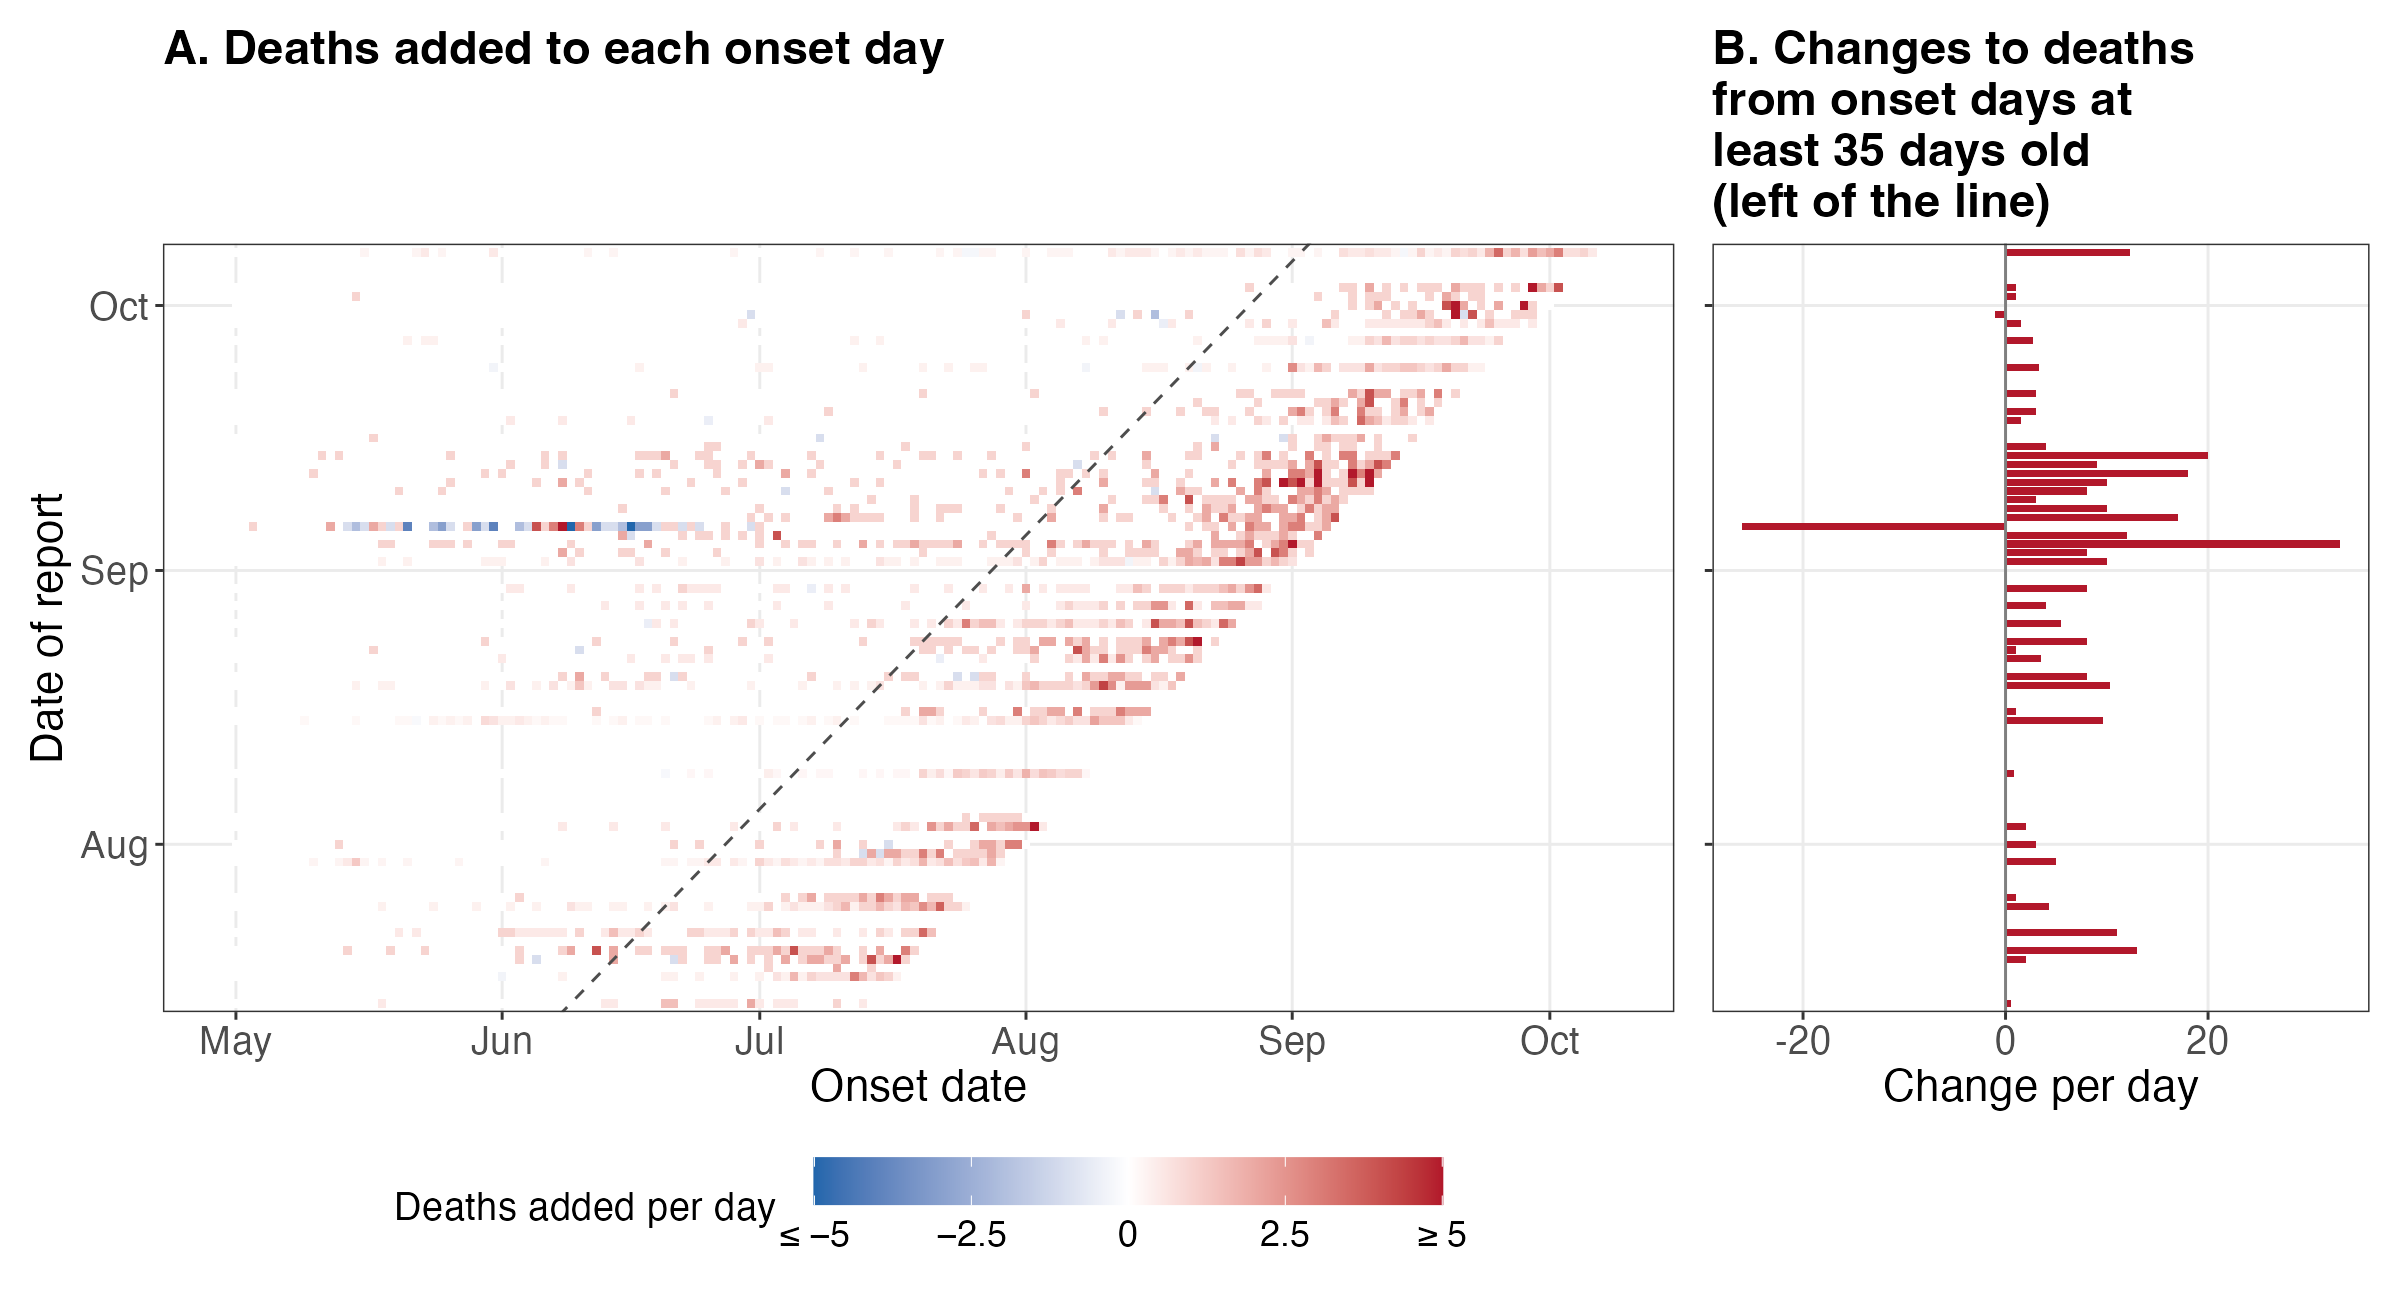
\includegraphics[height=0.74\textheight]{bvd_deaths_increments.png}

\smallskip
{\small Each situation report revises the deaths for every onset date, and
goes on adding deaths to onset days months old: most in bursts, in early
September. (6 September: a report which corrected many records.)}
\end{frame}

% ---------------------------------------------------------------------------
\begin{frame}{Recap: the model of cases}
Each report gives $C(t\given t_j)$: confirmed cases with onset on day $t$, as
known on day $t_j$. The true cases $I(t)$ are unknown.

\bigskip
\textbf{Transmission.} A renewal process with overdispersion:
\[
I(t)\sim\operatorname{NB}\bigl(R_t\,\Lambda_t,\ \kappa\bigr),\qquad
\Lambda_t=\sum_{s=1}^{40}\omega_s\,I(t-s)
\]

\textbf{Reporting.} Each case is reported after a gamma$(\mu,\sigma)$ delay,
with each day's hazard multiplied by an effect of the day of the week.
$S^{C}(t\given t')$: probability a case is not yet reported at $t'$.
\[
\Delta C(t\given t_j)\sim\bin\Bigl(I(t)-C(t\given t_{j-1}),\
1-\frac{S^{C}(t\given t_j)}{S^{C}(t\given t_{j-1})}\Bigr)
\]
\end{frame}

% ---------------------------------------------------------------------------
\begin{frame}{Recap: the model of cases}
\textbf{Wrong records.} Counts sometimes fall. Records are added in error
in proportion to reporting activity (rate $\eta$), and each is removed with
probability $\rho$ a day.

\bigskip
\textbf{Changes at unknown times.} $R_t$ and $(\mu,\sigma)$ are constant
within segments of onset days. Each day starts a new segment with
probability $p\sim\operatorname{beta}(1,T)$; the number of changes is
inferred.

\bigskip
\textbf{Fitting.} Metropolis within Gibbs: $I(t)$ from its discrete full
conditional, $R_t$ segments drawn exactly with their values integrated out,
the delay segments by split, merge and shift moves.

\bigskip
Today: adding deaths to this.
\end{frame}

% ---------------------------------------------------------------------------
\begin{frame}{What the reports show}
Each report splits each onset day's cases into alive and dead. For onset
day $t$ and the report of day $t_j$:
\begin{align*}
C(t\given t_j) &: \text{confirmed cases counted for day $t$};\\
D(t\given t_j) &: \text{the number of those cases shown as dead},\quad D\le C.
\end{align*}

\begin{itemize}
\item \textbf{No dates of death.} A death is counted on the reported onset
day of its case.
\item \textbf{Deaths are shown only with their cases.} A case can first
appear already dead.
\item \textbf{Deaths lag cases.} At 7 to 14 days after onset the case count
is about 79\% of its latest value, and the death count about 60\%.
\end{itemize}
\end{frame}

% ---------------------------------------------------------------------------
\begin{frame}{Approach}
Unknown for each onset day: the true cases $I(t)$ and, of those, the cases
which will die, $F(t)\le I(t)$:
\[
p\bigl(I, F, R, \cfr, \theta, \phi \given C, D\bigr)\;\propto\;
\underbrace{p\bigl(C, D\given I, F, \theta, \phi\bigr)}_{\text{reporting}}\;
\underbrace{p\bigl(F\given I, \cfr\bigr)}_{\text{fatality}}\;
\underbrace{p\bigl(I\given R\bigr)}_{\text{transmission}}\;
p(R)\,p(\cfr)\,p(\theta)\,p(\phi)
\]

\bigskip
\begin{itemize}
\item $\cfr_t$: case fatality ratio, by onset day. $F(t)\sim\bin\bigl(I(t),\cfr_t\bigr)$.
\item $\theta$: the vector of parameters of the reporting of cases, as
before (delay, day-of-week effects, wrong records).
\item $\phi$: the vector of parameters of the recording of deaths (delay,
day-of-week effects, and those introduced on later slides).
\item $\cfr_t$ and the delay to a death being recorded each have their own
change points, with the same model for them as for $R_t$.
\end{itemize}

\bigskip
Aims: to estimate the eventual numbers of cases and of deaths for recent
onset days, and $\cfr_t$, allowing for deaths not yet recorded.
\end{frame}

% ---------------------------------------------------------------------------
\begin{frame}{Two delays for each fatal case}
We are building up to a more nuanced delay model but, to start, let's
assume that the following delays from onset are independent:

\smallskip
\begin{center}
\renewcommand{\arraystretch}{1.3}
\begin{tabular}{lll}
\toprule
 & Delay & Probability it has not happened by $t'$ \\
\midrule
The case is reported & $T_C$ & $S^{C}(t\given t')$ \\
The death is recorded & $T_D$ & $S^{D}(t\given t')$ \\
\bottomrule
\end{tabular}
\end{center}

\medskip
\begin{itemize}
\item A fatal case is shown as dead once it is reported \emph{and}
its death is recorded.
\item Reported, but death not yet recorded: shown as alive.
\item So some of the cases shown as alive will die, and we cannot see which because we do
not have a line list.
\end{itemize}

\bigskip
Later slides change this: a death can bring about the report of its case
($T_C$ and $T_D$ then depend on each other), and $T_D$ becomes the time to death
plus a delay to recording.
\end{frame}

% ---------------------------------------------------------------------------
\begin{frame}{What a report shows}
The cases of onset day $t$ in the report of $t_j$ are of three kinds:

\medskip
\begin{center}
\renewcommand{\arraystretch}{1.4}
\begin{tabular}{lll}
\toprule
 & Number & Shown as \\
\midrule
Non-fatal cases reported so far & $C^{N}(t\given t_j)$ & alive \\
Fatal cases reported, death not yet recorded & $C^{F}(t\given t_j)-D(t\given t_j)$ & alive \\
Fatal cases reported, death recorded & $D(t\given t_j)$ & dead \\
\bottomrule
\end{tabular}
\end{center}

\bigskip
\begin{itemize}
\item Observed: $C=C^{N}+C^{F}$ and $D$.
\item Not observed: the split of $C$ into $C^{F}$ and $C^{N}$.
\end{itemize}
\end{frame}

% ---------------------------------------------------------------------------
\begin{frame}{From one report to the next}
\begin{align*}
\text{fatal cases new to the report}\quad
 & \Delta C^{F}(t\given t_j)\sim\bin\bigl(F(t)-C^{F}(t\given t_{j-1}),\ p^{F}(t\given t_j)\bigr)\\[3pt]
\text{non-fatal cases new to the report}\quad
 & \Delta C^{N}(t\given t_j)\sim\bin\bigl(N(t)-C^{N}(t\given t_{j-1}),\ p^{N}(t\given t_j)\bigr)\\[3pt]
\text{new cases already shown as dead}\quad
 & \dnew(t\given t_j)\sim\bin\bigl(\Delta C^{F}(t\given t_j),\ p^{\text{dead}}(t\given t_j)\bigr)\\[3pt]
\text{cases shown as alive before, now dead}\quad
 & \dold(t\given t_j)\sim\bin\Bigl(C^{F}(t\given t_{j-1})-D(t\given t_{j-1}),\
 1-\frac{S^{D}(t\given t_j)}{S^{D}(t\given t_{j-1})}\Bigr)
\end{align*}

\smallskip
Observed: $\Delta C=\Delta C^{F}+\Delta C^{N}$ and $\Delta D=\dnew+\dold$.

\medskip
\begin{itemize}
\item $p^{F}(t\given t_j)$: probability a fatal case not in the report of
$t_{j-1}$ is in that of $t_j$.
\item $p^{N}(t\given t_j)$: the same for a non-fatal case. With independent
delays, $p^{F}=p^{N}=1-S^{C}(t\given t_j)/S^{C}(t\given t_{j-1})$.
\item $p^{\text{dead}}(t\given t_j)$: probability a fatal case new to the
report of $t_j$ is already shown as dead in it. With independent delays,
$p^{\text{dead}}=1-S^{D}(t\given t_j)$.
\end{itemize}
\end{frame}

% ---------------------------------------------------------------------------
\begin{frame}{Wrong records}
Counts of cases sometimes fall, and so do counts of deaths (18 times in
2{,}129 comparisons of consecutive reports, never by more than 2). So, as for
cases, some records are wrong, and now each is shown as alive or as dead:
\[
C(t\given t_j)=C^{N}+C^{F}+E^{A}+E^{D},\qquad
D(t\given t_j)=D^{F}+E^{D},
\]
where $D^{F}$ is the genuine fatal cases shown as dead (the $D$ of the
previous slides).

\medskip
Between the reports of $t_{j-1}$ and $t_j$, for onset day $t$:
\begin{align*}
\text{wrong records added, shown as alive}\quad & \operatorname{Poisson}\bigl((1-\delta)\,\lambda_j\bigr)\\
\text{wrong records added, shown as dead}\quad & \operatorname{Poisson}\bigl(\delta\,\lambda_j\bigr),\qquad
\lambda_j=\eta\times\text{expected genuine cases newly reported}\\
\text{each wrong record present is removed}\quad & \text{with probability }1-(1-\rho)^{t_j-t_{j-1}}
\end{align*}

\begin{itemize}
\item Errors are made when cases are being reported, and are found later.
\item A fall in deaths with no fall in cases: a wrong record shown as dead is
removed while a genuine case is added.
\item $\delta\sim\operatorname{beta}(1,1)$; $\eta$ and $\rho$ as for cases.
\item The hidden counts in each report are now $C^{F}$, $E^{A}$ and $E^{D}$.
\end{itemize}
\end{frame}

% ---------------------------------------------------------------------------
\begin{frame}{A puzzle: deaths shown very early}
For each onset day and each report, take the cases of that onset day shown
in the report and the share of them shown as dead. Group by the days from
onset to report (onset days 12 July to 5 September):

\medskip
\begin{center}
\small
\renewcommand{\arraystretch}{1.15}
\begin{tabular}{ccc}
\toprule
Days from & Cases shown & Share shown \\
onset to report & (summed over reports) & as dead \\
\midrule
0--1 & 148 & 0.43 \\
2--7 & 3,970 & 0.35 \\
8--14 & 10,850 & 0.37 \\
15--28 & 27,014 & 0.41 \\
29--42 & 28,766 & 0.44 \\
43 or more & 39,158 & 0.46 \\
\bottomrule
\end{tabular}
\end{center}

If $T_C$ and $T_D$ were independent, this share would be about
$\cfr_t\,[1-S^{D}(u)]$ at $u$ days: near zero at first, then rising.
Instead, it starts high (0.43), dips, then rises again.
\end{frame}

% ---------------------------------------------------------------------------
\begin{frame}{A puzzle: deaths shown very early}
\begin{itemize}
\item To fit this with independent delays, $T_D$ needs a spike near zero and
a very long tail (gamma shape about 0.2, mean 46 days).
\item It then expects many deaths still to come, and overshoots badly.
\end{itemize}

\bigskip
There are two potential explanations we consider in what follows for these
patterns: a person dying actually triggers a case to be reported or some
proportion of cases that die have their date of onset recorded as their date
of death.
\end{frame}

% ---------------------------------------------------------------------------
\begin{frame}{Explanation 1: a death which brings about the report}
A share $\tau$ of fatal cases are reported when their death is recorded, if
they have not been reported by then:
\[
\text{time to being reported}=
\begin{cases}
\min(T_C,T_D) & \text{with probability } \tau\\
T_C & \text{with probability } 1-\tau
\end{cases}
\]

A fatal case is not yet reported at $t'$ with probability
\[
M(t\given t')=S^{C}(t\given t')\,\bigl[(1-\tau)+\tau\,S^{D}(t\given t')\bigr],
\qquad
p^{F}(t\given t_j)=1-\frac{M(t\given t_j)}{M(t\given t_{j-1})}.
\]

\begin{itemize}
\item Fatal cases are reported sooner than others, and early reports are
more often fatal.
\item Only $p^{F}$ and $p^{\text{dead}}$ change, so the likelihood keeps
the same form.
\item $\tau=0$ is the independent model. $\tau\sim\operatorname{beta}(1,1)$.
\end{itemize}
\end{frame}

% ---------------------------------------------------------------------------
\begin{frame}{Explanation 2: some onset dates are incorrectly recorded as the date of death}
Some fatal cases may be identified only at or after death, and have their
date of death recorded as their onset date.

\bigskip
\begin{itemize}
\item Such a case is counted about nine days later than its true onset, and
can be shown as dead almost at once.
\item To tell how many there are, we need what is known of the true time
from onset to death (next slide).
\item The reports describe the curve as by date of onset: whether some are
by date of death is an inference, not something the reports say.
\end{itemize}
\end{frame}

% ---------------------------------------------------------------------------
\begin{frame}{The time from onset to death}
\centering
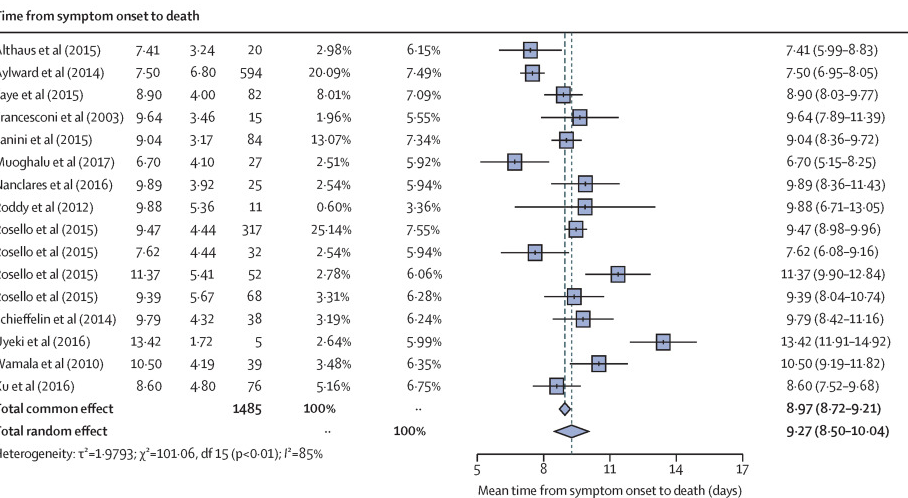
\includegraphics[height=0.72\textheight]{bvd_onset_to_death_review.png}

\smallskip
{\small Nash et al.\ (2024, \emph{Lancet Infect.\ Dis.}). We assume a
gamma(mean 9.3, sd 5.5 days): the random-effects mean, and the studies' sds
weighted by patients.}
\end{frame}

% ---------------------------------------------------------------------------
\begin{frame}{Are the deaths in the reports consistent with this?}
Deaths shown within 1 and 2 days of their recorded onset day:

\medskip
\begin{center}
\renewcommand{\arraystretch}{1.3}
\begin{tabular}{lcc}
\toprule
 & Within 1 day & Within 2 days \\
\midrule
Expected if every onset were correctly dated: & & \\
\quad deaths by then, gamma (mean 9.3, sd 5.5) & 0.5\% & 3\% \\
In the reports: share of the deaths eventually & & \\
\quad recorded for a day already shown by then & 7.8\% & 14\% \\
\bottomrule
\end{tabular}
\end{center}

\medskip
\begin{itemize}
\item The expected values are upper bounds: a death must also be recorded,
and its case reported, before it is shown.
\item So, with this time from onset to death, the early deaths can only be
cases whose onset was recorded as their date of death: we call them
misdated. Their number says what fraction $f$ of fatal cases are
misdated.
\end{itemize}
\end{frame}

% ---------------------------------------------------------------------------
\begin{frame}{Misdated cases: two sets of counts}
$I(t)$, $F(t)$ and $\cfr_t$ stay by true day of onset, so transmission
and the case fatality ratio are on the right days. Of the fatal cases with
true onset on day $t$,
\[
F^{\mathrm{mis}}(t)\sim\bin\bigl(F(t),\ f\bigr),\qquad f\sim\operatorname{beta}(1,1),
\]
are misdated: recorded on their day of death, $Z\sim h$ days later
($Z\ge1$; the supplied gamma, discretised). $F^{\mathrm{mis}}(t,z)$: those
who die $z$ days after onset (multinomial given $F^{\mathrm{mis}}(t)$).

\bigskip
The reports count, for day $t$,
\[
\tilde{F}(t)=\underbrace{F(t)-F^{\mathrm{mis}}(t)}_{\text{true onset on day }t}
+\underbrace{G(t)}_{\substack{\text{misdated:}\\\text{died on day }t}},\qquad
G(t)=\sum_{z\ge1}F^{\mathrm{mis}}(t-z,z).
\]

\bigskip
{\small Example: 10 fatal cases with true onset on 9 August, 4 of them
misdated; 5 misdated cases with earlier onsets die on 9 August. Then
$\tilde{F}=10-4+5=11$.}
\end{frame}

% ---------------------------------------------------------------------------
\begin{frame}{Misdated cases: an approximation}
The exact likelihood would follow correctly dated and misdated fatal cases
($C^{F,\mathrm{onset}}$ and $C^{F,\mathrm{mis}}$) separately: two hidden
counts per day and report, and several times slower.

\bigskip
Instead, each of the $\tilde{F}(t)$ fatal cases recorded for day $t$ is
taken to be misdated with probability $\tilde{f}_t=G(t)/\tilde{F}(t)$,
independently. Not yet reported at $t'$:
\[
\tilde{M}(t\given t')=(1-\tilde{f}_t)\,M(t\given t')+\tilde{f}_t\,S^{U}(t\given t')
\]

\begin{itemize}
\item A misdated case enters the records when its death does ($S^{U}$, next
slides), and is shown as dead from the start.
\item The hidden count stays $C^{F}$ alone.
\item Expected counts in each report are the same as in the exact version;
the approximation allows somewhat more variation about them. Checked on
data simulated exactly.
\end{itemize}
\end{frame}

% ---------------------------------------------------------------------------
\begin{frame}{The delay to a death being recorded}
With onset to death supplied, $T_D=Z+U$: the time to death, then a delay $U$
from death to the death being recorded, gamma$(\mu^{d},\sigma^{d})$:
\[
S^{D}(t\given t')=\sum_{z>t'-t}h_z+\sum_{z\le t'-t}h_z\,S^{U}(t+z\given t')
\]

\begin{itemize}
\item $(\mu^{d},\sigma^{d})$ are estimated, and can change at unknown
times; $h$ is fixed.
\item Effects of the day of the week act on the hazard of recording.
\item A death cannot be shown on the day of onset.
\end{itemize}

\bigskip
\textbf{What $f$ rests on.} Mostly the sd of the time to death: a wider $h$
allows more early deaths among correctly dated cases. A rough fit gives
$f$ of 0.40, 0.33, 0.26 and 0.17 for sds of 4.5, 5.5, 6.5 and 8 days.
\end{frame}

% ---------------------------------------------------------------------------
\begin{frame}{Deaths recorded long after}
With the time to death near nine days, a death first shown months after
onset must be explained by $U$. A gamma with a mean of a few days makes such
deaths all but impossible.

\bigskip
So a share $\omega^{d}$ of deaths are recorded after an exponential delay
with mean $m^{d}$ instead (the \emph{recording tail}):
\[
S^{U}(d\given t')=(1-\omega^{d})\,S_{\mathrm{gamma}}(t'-d\given\mu^{d},\sigma^{d})
+\omega^{d}\,e^{-(t'-d)/m^{d}}
\]

\begin{itemize}
\item $\omega^{d}\sim\operatorname{beta}(1,9)$; $m^{d}\sim$ gamma with mean
40 and sd 20 days.
\item Both are the same for all onset days.
\item This is where most of the difficulty lies (later slides).
\end{itemize}
\end{frame}

% ---------------------------------------------------------------------------
\begin{frame}{Changes at unknown times}
Four quantities are piecewise constant in the onset day, each with its own
change points and the same prior on them.

\bigskip
\begin{center}
\renewcommand{\arraystretch}{1.35}
\begin{tabular}{lll}
\toprule
Quantity & Prior within a segment & Minimum segment \\
\midrule
$R_t$ & gamma & 7 days \\
Reporting delay $(\mu,\sigma)$ & hierarchical log-normal & 14 days \\
Case fatality ratio $\cfr_t$ & $\operatorname{beta}(1,1)$ & 14 days \\
Recording delay $(\mu^{d},\sigma^{d})$ & hierarchical log-normal & 14 days \\
\bottomrule
\end{tabular}
\end{center}

\bigskip
\begin{itemize}
\item $\cfr_t$ is indexed by onset day: a change is between cohorts of cases.
\item Onset days first seen long after onset (to 18 July) cannot show how
fast deaths were recorded, so they share one recording delay.
\end{itemize}
\end{frame}

% ---------------------------------------------------------------------------
\begin{frame}{Inference method}
Metropolis within Gibbs, extending the sampler for cases. We infer:

\medskip
\begin{center}
\small
\renewcommand{\arraystretch}{1.3}
\begin{tabular}{lp{0.62\textwidth}}
\toprule
\multicolumn{2}{l}{\textbf{Counts, for each onset day $t$}}\\
$I(t)$, $F(t)$ & true cases, and the fatal cases among them\\
$F^{\mathrm{mis}}(t,z)$ & fatal cases of true onset day $t$, misdated to
their day of death $t+z$\\
$C^{F}$, $E^{A}$, $E^{D}$ & hidden counts in each report $t_j$: fatal cases,
and wrong records shown as alive and as dead\\
\midrule
\multicolumn{2}{l}{\textbf{Parameters}}\\
Transmission & $R_t$ (with change points), $\kappa$\\
Reporting of cases, $\theta$ & $(\mu,\sigma)$ (with change points), $\psi_w$, $\eta$, $\rho$\\
Fatality & $\cfr_t$ (with change points)\\
Recording of deaths, $\phi$ & $(\mu^{d},\sigma^{d})$ (with change points),
$\psi^{d}_w$, $\omega^{d}$, $m^{d}$, $\tau$, $f$, $\delta$; report effects
$\varepsilon_j$ and $s$ in some options\\
\bottomrule
\end{tabular}
\end{center}

\medskip
Write $y_t=\{C(t\given t_j),D(t\given t_j)\}_{j=1}^{J}$: the counts of cases
and of deaths for onset day $t$ in every report.
\end{frame}

% ---------------------------------------------------------------------------
\begin{frame}{Inference method}
\textbf{The counts of each onset day.} We can calculate
$p\bigl(y_t\given I(t),F(t),\theta,\phi\bigr)$ exactly, summing over the hidden
counts $C^{F}$, $E^{A}$, $E^{D}$ in every report. Each sweep, for each $t$:

\medskip
\begin{enumerate}
\item $F(t)$, with the hidden counts summed out: propose $F'=F(t)\pm k$, $k\in\{1,2,3\}$,
and accept with probability
\[
\min\Bigl\{1,\ \frac{p(y_t\given I(t),F')\,\bin\bigl(F'\given I(t),\cfr_t\bigr)\,
\bin\bigl(F^{\mathrm{mis}}(t)\given F',f\bigr)}
{p(y_t\given I(t),F(t))\,\bin\bigl(F(t)\given I(t),\cfr_t\bigr)\,
\bin\bigl(F^{\mathrm{mis}}(t)\given F(t),f\bigr)}\Bigr\}.
\]
\item The hidden counts are drawn exactly from their conditional given $y_t$,
$I(t)$ and $F(t)$: those in the last report first, then those in each
earlier report given the later ones.
\item $I(t)$ is drawn exactly from its discrete conditional, with $F(t)$
summed out:
\[
p\bigl(I(t)\given\cdot\bigr)\propto\prod_{s\ge t}\operatorname{NB}\bigl(I(s)\given R_s\Lambda_s,\kappa\bigr)
\sum_{F}\bin\bigl(F\given I(t),\cfr_t\bigr)\,\bin\bigl(F^{\mathrm{mis}}(t)\given F,f\bigr)\,
p\bigl(y_t,C^{F},E^{A},E^{D}\given I(t),F\bigr).
\]
\item $F(t)$ is drawn exactly given $I(t)$ and the hidden counts: the summand above,
normalised over $F$.
\end{enumerate}
\end{frame}

% ---------------------------------------------------------------------------
\begin{frame}{Inference method}
\textbf{Which fatal cases are misdated.} Metropolis proposals change the
counts $F^{\mathrm{mis}}(t,z)$ by one, keeping the number of fatal cases
recorded for each day, $\tilde{F}$, fixed:
\begin{itemize}
\item one of the fatal cases recorded for day $s$ switches between ``onset on
day $s$'' and ``onset on day $s-z$, misdated to its day of death $s$'': $I$ and
$F$ change by one on both days;
\item one misdated to its day of death $s$ is given a different time to death
$z'$: it moves from onset day $s-z$ to $s-z'$.
\end{itemize}
The ratio includes the renewal model, $h$, $\bin(F^{\mathrm{mis}}\given F,f)$ and
$p(y\given I,F)$ for the days changed.

\medskip
\textbf{Parameters.}
\begin{itemize}
\item $\cfr_t$: change points drawn with the values integrated out
(beta-binomial), as for $R_t$; then for each segment $k$,
$\cfr_k\sim\operatorname{beta}\bigl(1+\sum_{t\in k}F(t),\ 1+\sum_{t\in k}[I(t)-F(t)]\bigr)$.
\item $f$: close to $\operatorname{beta}\bigl(1+\sum_tF^{\mathrm{mis}}(t),\
1+\sum_t[F(t)-F^{\mathrm{mis}}(t)]\bigr)$; drawn from a beta matched to its conditional,
with a Metropolis--Hastings correction.
\item $\delta$ and $\eta$: conjugate (beta and gamma), given the wrong records
in $H$.
\item $(\mu,\sigma)$ and $(\mu^{d},\sigma^{d})$: split, merge and shift moves
of change points.
\item $\kappa$, $\rho$, $\tau$, $\omega^{d}$, $m^{d}$, $\psi_w$, $\psi^{d}_w$:
random-walk Metropolis.
\end{itemize}
\end{frame}

% ---------------------------------------------------------------------------
\begin{frame}{What can and cannot be learned}
\begin{itemize}
\item \textbf{A recent fall in $\cfr_t$ and deaths not yet recorded look the
same.} For the last three to four weeks of onset days, $\cfr_t$ rests mostly on
the recording delay estimated from earlier days.
\item \textbf{A change in the recording delay and in $\cfr_t$ at about the same
time are hard to tell apart.}
\item \textbf{$f$ rests on the supplied time to death,} and misdated cases who
have yet to die are in no report.
\item \textbf{Old onset days say little about the reporting delay of cases,
but much about deaths,} which go on being recorded for weeks.
\end{itemize}
\end{frame}

% ---------------------------------------------------------------------------
\begin{frame}{Fits to past sitreps: deaths}
\centering
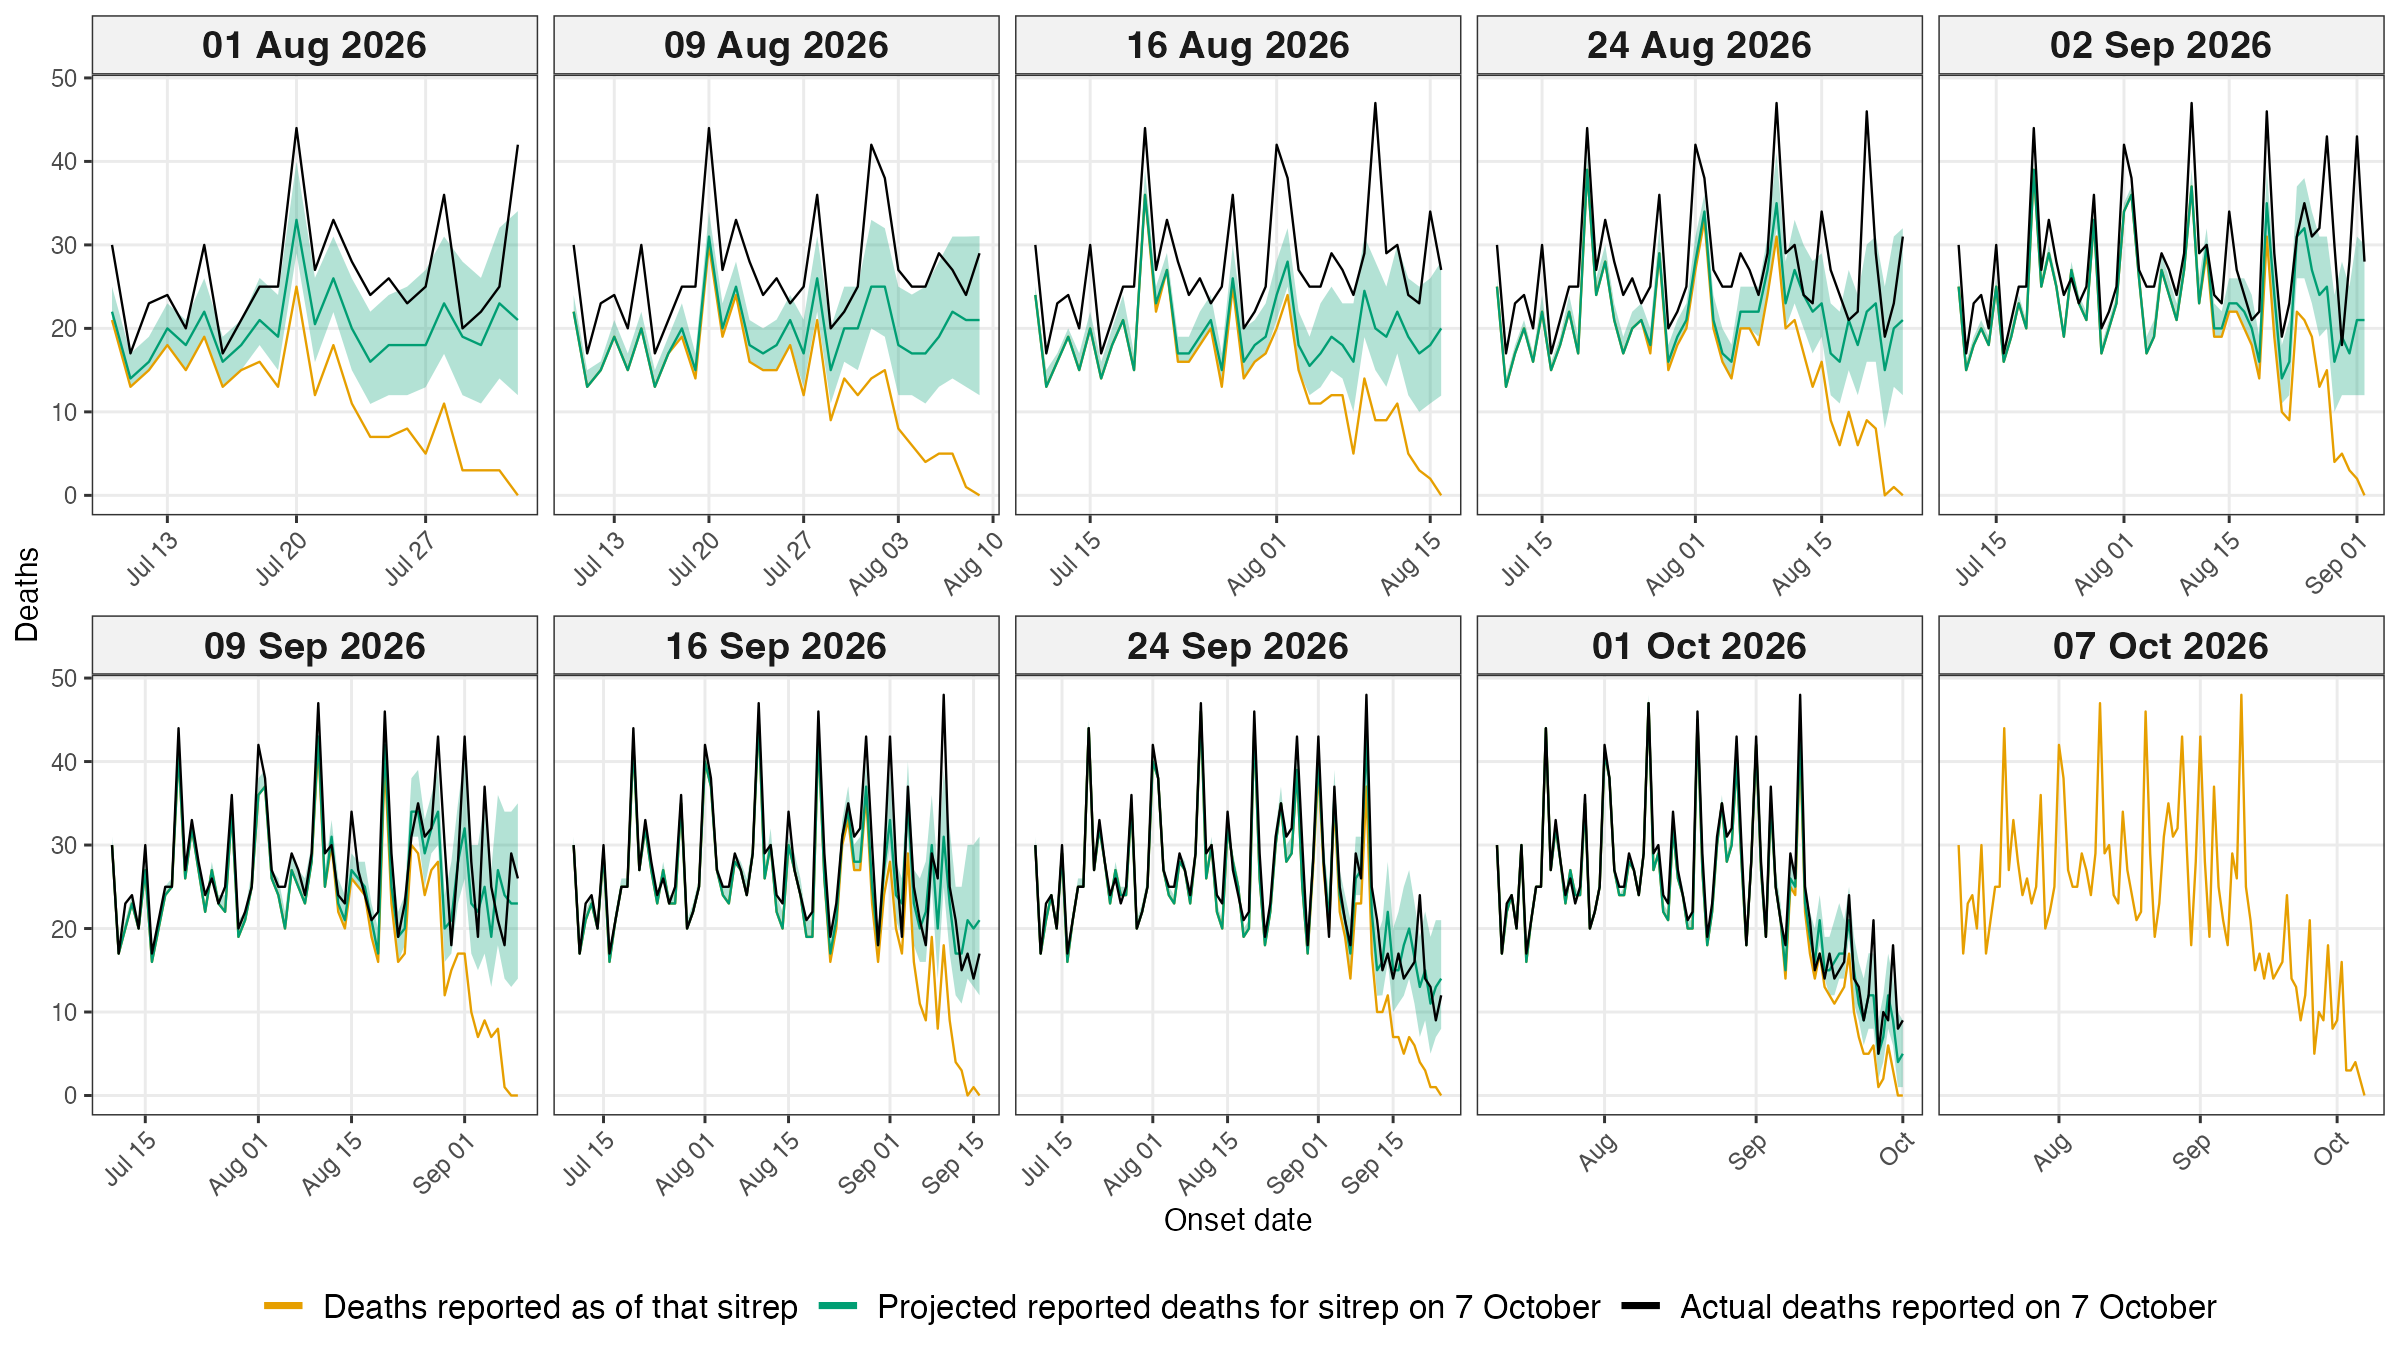
\includegraphics[height=0.8\textheight]{bvd_deaths_fits_deaths.png}

{\small Panels: the date of each fit. Shading: 90\% interval of the projection.}
\end{frame}

% ---------------------------------------------------------------------------
\begin{frame}{Fits to past sitreps: deaths in the latest 28 onset days}
\centering
\renewcommand{\arraystretch}{1.2}
\begin{tabular}{lcccc}
\toprule
 & \multicolumn{3}{c}{Deaths} & \\
\cmidrule(lr){2-4}
Fit date & Shown then & Projected for 7 Oct & Shown 7 Oct & Share in the tail, $\omega^{d}$ \\
\midrule
1 Aug & 348 & 796 (681--893) & 709 & 0.56 \\
9 Aug & 380 & 728 (660--844) & 761 & 0.47 \\
16 Aug & 403 & 632 (581--732) & 813 & 0.47 \\
24 Aug & 441 & 687 (639--776) & 798 & 0.50 \\
2 Sep & 495 & 782 (728--844) & 826 & 0.54 \\
9 Sep & 489 & 871 (747--975) & 786 & 0.46 \\
16 Sep & 513 & 840 (758--909) & 768 & 0.46 \\
24 Sep & 457 & 662 (625--710) & 639 & 0.32 \\
1 Oct & 379 & 490 (471--512) & 510 & 0.30 \\
\bottomrule
\end{tabular}

\medskip
\begin{minipage}{0.88\textwidth}
\small Posterior medians and 90\% intervals. Up to 2 September the
projections are mostly too low; on 9 and 16 September they are about 10\%
too high.
\end{minipage}
\end{frame}

% ---------------------------------------------------------------------------
\begin{frame}{Deaths are added to old onset days in bursts}
\centering
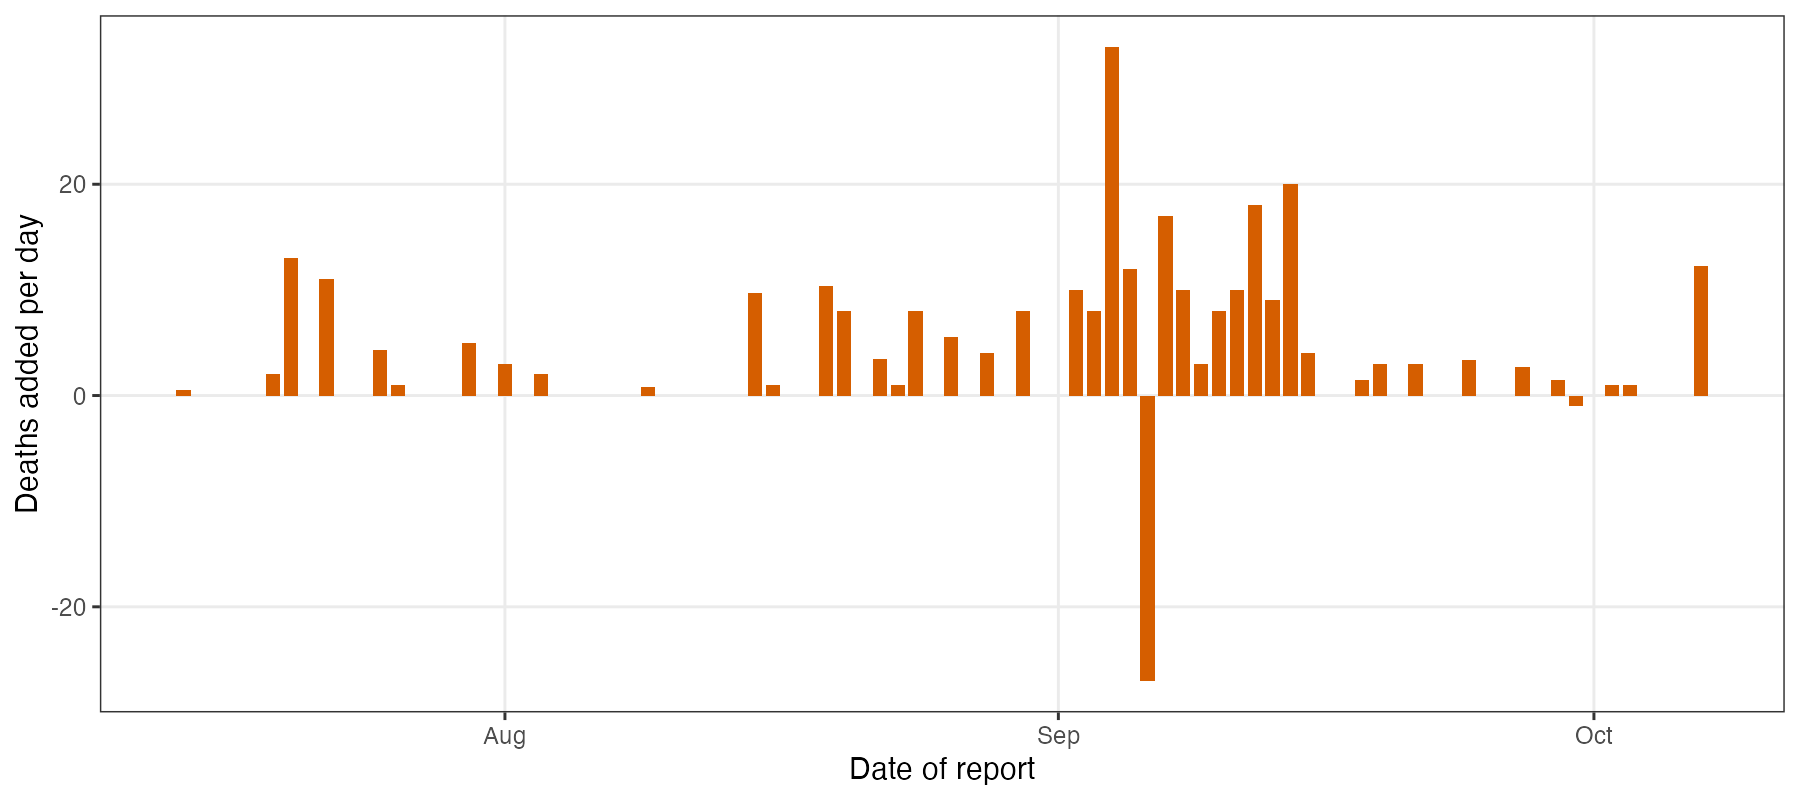
\includegraphics[height=0.6\textheight]{bvd_deaths_late_additions.png}

\smallskip
\begin{minipage}{0.85\textwidth}
\small Deaths added by each report to onset days at least 35 days old, per
day since the report before. (6 September: a report which corrected many
records.)
\end{minipage}
\end{frame}

% ---------------------------------------------------------------------------
\begin{frame}{Two ways to explain the late deaths}
From 9 September, the posterior has two modes:

\bigskip
\begin{center}
\renewcommand{\arraystretch}{1.35}
\begin{tabular}{lcc}
\toprule
 & Heavy tail & Light tail \\
\midrule
Share of deaths in the tail, $\omega^{d}$ & about 0.45 & about 0.15 \\
Mean of the tail, $m^{d}$ & about 40 days & -- \\
Recording delay, early onset days & about 2.5 days & about 20 days, then changes \\
Case fatality ratio, latest onset days & 0.60 to 0.65 & about 0.5 \\
\bottomrule
\end{tabular}
\end{center}

\bigskip
\begin{itemize}
\item The heavy tail expects the September bursts to go on: projections
too high.
\item The light tail explains them by a slow early delay and changes in it.
\item Both are features of onset days; the bursts are features of reports.
\end{itemize}
\end{frame}

% ---------------------------------------------------------------------------
\begin{frame}{Options for the recording delay}
\begin{center}
\renewcommand{\arraystretch}{1.4}
\begin{tabular}{lp{0.62\textwidth}}
\toprule
Option & Recording delay $(\mu^{d},\sigma^{d})$ \\
\midrule
Base & Changes at unknown times; fixed for onset days to 18 July \\
(a) & Fixed for onset days to 31 July, then changes at unknown times \\
(b) & One delay for all onset days \\
(c) & As base, and each report has its own effect on recording \\
(d) & As (b), and each report has its own effect on recording \\
(e) & As (b), and each report has its own effect on the tail alone \\
(f) & As (a), and each report has its own effect on the tail alone \\
\bottomrule
\end{tabular}
\end{center}

\bigskip
(a) and (b) remove freedom the data seem not to use. (c) to (f) let the
bursts be bursts, rather than features of onset days.
\end{frame}

% ---------------------------------------------------------------------------
\begin{frame}{Effects of each report on recording}
The hazard of a death being recorded on each day after report $t_{j-1}$, up
to and including report $t_j$, is multiplied by
\[
\psi^{d}_{w(j)}\,e^{\varepsilon_j},\qquad
\varepsilon_j\sim N(0,s^2),\qquad s^2\sim\operatorname{inverse\ gamma}(3,\,0.2),
\]
with $w(j)$ the day of the week of report $t_j$.

\bigskip
\begin{itemize}
\item One effect per report, shared by all onset days.
\item In (e) and (f), only the exponential tail is multiplied; the gamma
part keeps the day-of-week effects alone. A burst then clears a backlog of
old deaths without speeding up the deaths of recent onset days.
\item Reports after the fit date: effects are drawn from $N(0,s^2)$ when
projecting.
\item Sampled in blocks with steps scaled by $s$, with $s$ by Gibbs, and a
joint rescaling of $(\varepsilon,s)$ to cross the funnel.
\end{itemize}
\end{frame}

% ---------------------------------------------------------------------------
\begin{frame}{Effects of each report: the fit to 16 September, option (c)}
\centering
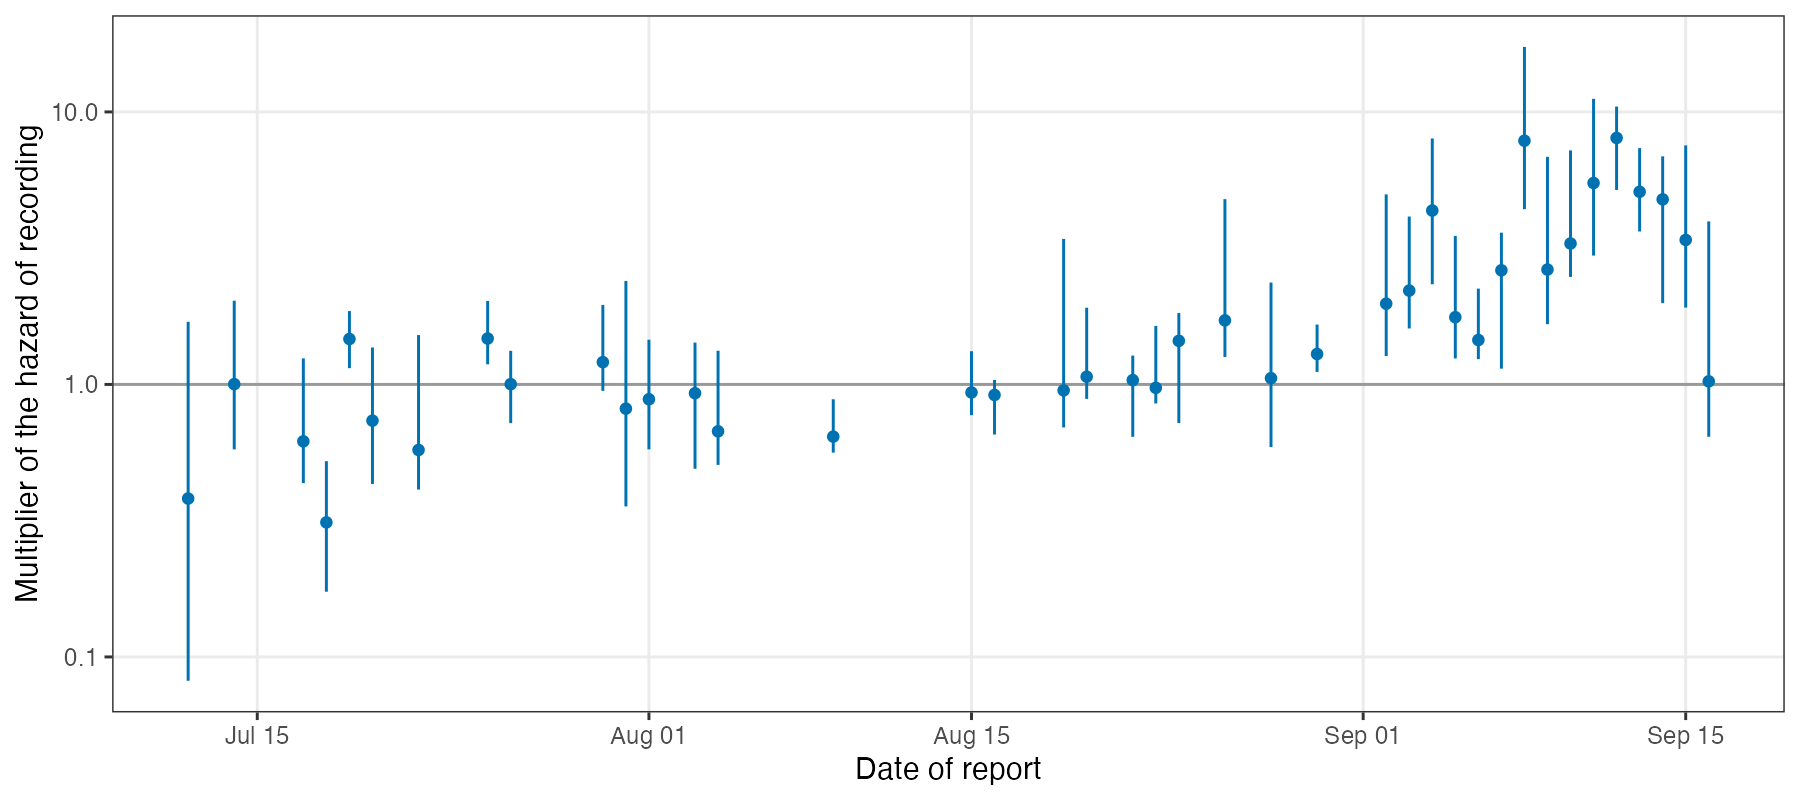
\includegraphics[height=0.62\textheight]{bvd_deaths_report_effects.png}

\smallskip
\begin{minipage}{0.85\textwidth}
\small Posterior medians and 90\% intervals. Multipliers of 2 to 8 on the
reports of 2 to 15 September, the bursts; near 1 otherwise. $s=0.88$
(0.73--1.10).
\end{minipage}
\end{frame}

% ---------------------------------------------------------------------------
\begin{frame}{The options compared: the fit to 16 September}
Deaths in the latest 28 onset days: 513 shown on 16 September, 768 on
7 October.

\medskip
\begin{center}
\renewcommand{\arraystretch}{1.3}
\begin{tabular}{lccc}
\toprule
Option & Projected for 7 Oct & Eventual & Case fatality ratio \\
\midrule
Base & 840 (758--909) & 1{,}081 (798--1{,}198) & 0.63 (0.48--0.70) \\
(a) Fixed to 31 July & 856 (812--906) & 1{,}104 (1{,}030--1{,}188) & 0.65 (0.60--0.69) \\
(b) One delay & 851 (803--906) & 1{,}098 (1{,}022--1{,}194) & 0.64 (0.60--0.70) \\
(c) Base, report effects & 692 (638--742) & 748 (700--790) & 0.46 (0.44--0.48) \\
(d) One delay, report effects & 676 (614--732) & 751 (651--798) & 0.47 (0.40--0.49) \\
\bottomrule
\end{tabular}
\end{center}

\medskip
\begin{itemize}
\item (a) and (b) choose the heavy tail: about 10\% too high.
\item (c) and (d) go too far the other way: their eventual deaths are fewer
than 7 October already shows. Effects on the whole delay speed up the
recording of recent deaths too. Hence (e) and (f).
\end{itemize}
\end{frame}

% ---------------------------------------------------------------------------
\begin{frame}{Where this leaves us}
\begin{itemize}
\item \textbf{Deaths bring reports, and some onset dates are recorded as
the date of death.} Both are needed to fit the early deaths with a plausible time to
death.
\item \textbf{The difficulty is the slow part of recording.} Bursts of late
deaths by report date can be explained in more than one way, and the fits
choose between them differently at different dates.
\item \textbf{Report effects remove the overshoot, but overcorrect}:
effects on the whole delay also speed up recent deaths.
\item \textbf{Next:} options (c) to (f) at every fit date from
1 August to 7 October, scored against the report of 7 October.
\item \textbf{Sensitivity:} the supplied time to death, especially its sd.
\end{itemize}
\end{frame}

% ---------------------------------------------------------------------------
\begin{frame}
\centering
\Huge Any questions?
\end{frame}

% ---------------------------------------------------------------------------
\appendix

\begin{frame}{Appendix: cases added by each report}
\centering
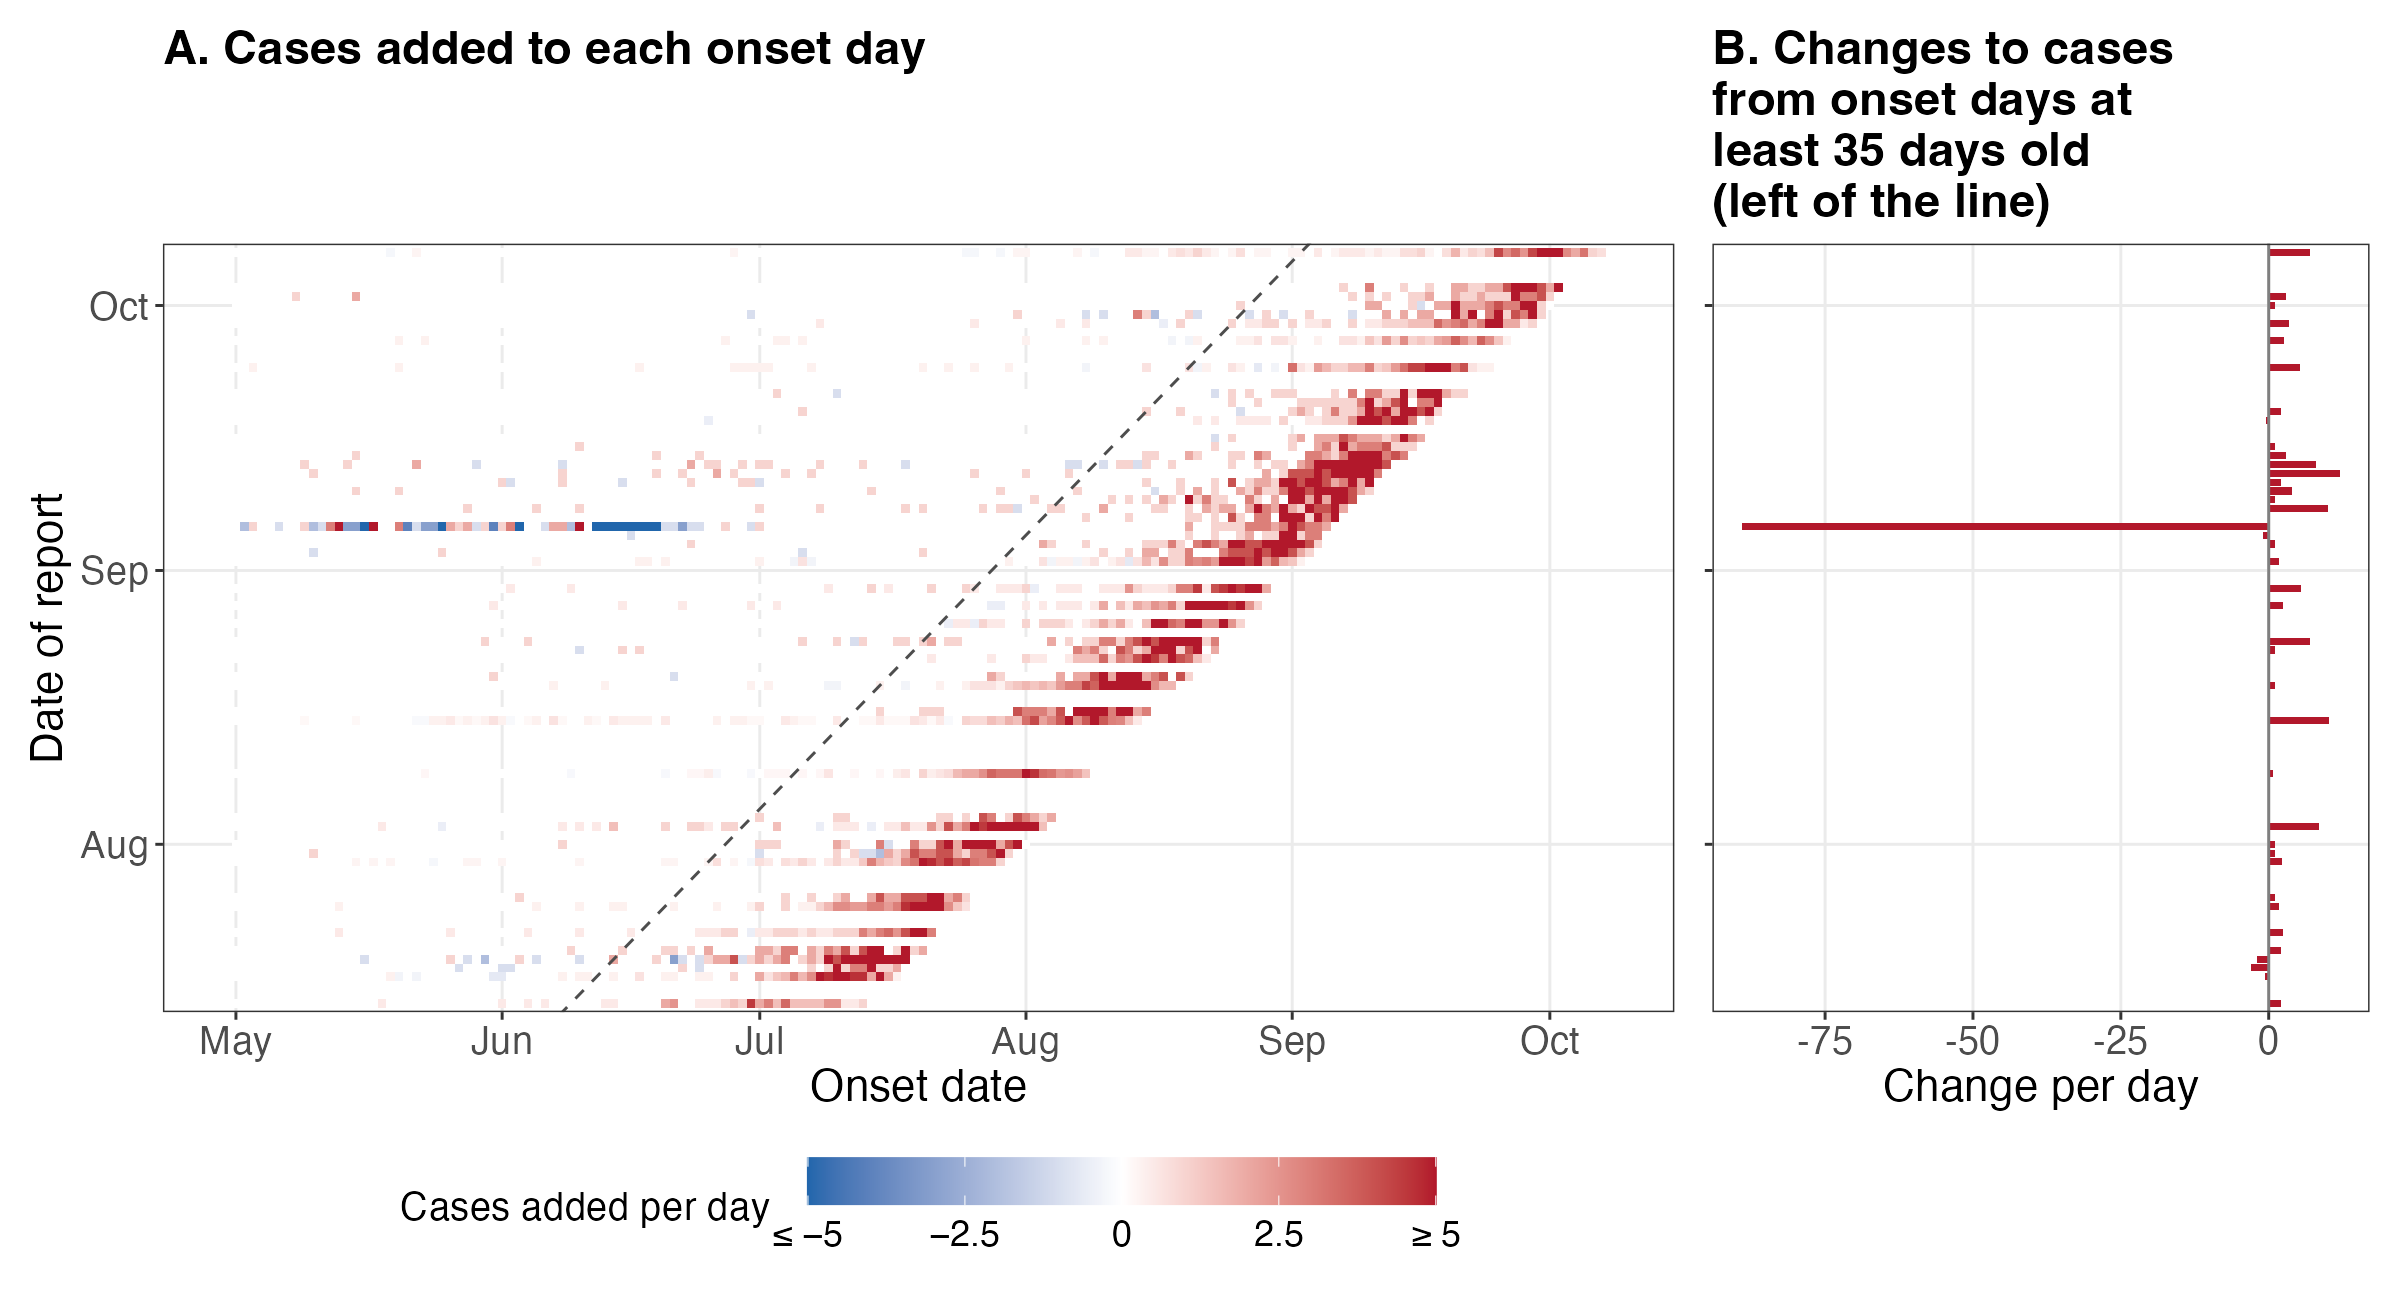
\includegraphics[height=0.74\textheight]{bvd_cases_increments.png}

\smallskip
{\small As the first slide, for cases. (6 September: a report which corrected
many records.)}
\end{frame}

\begin{frame}{Appendix: fits to past sitreps, cases}
\centering
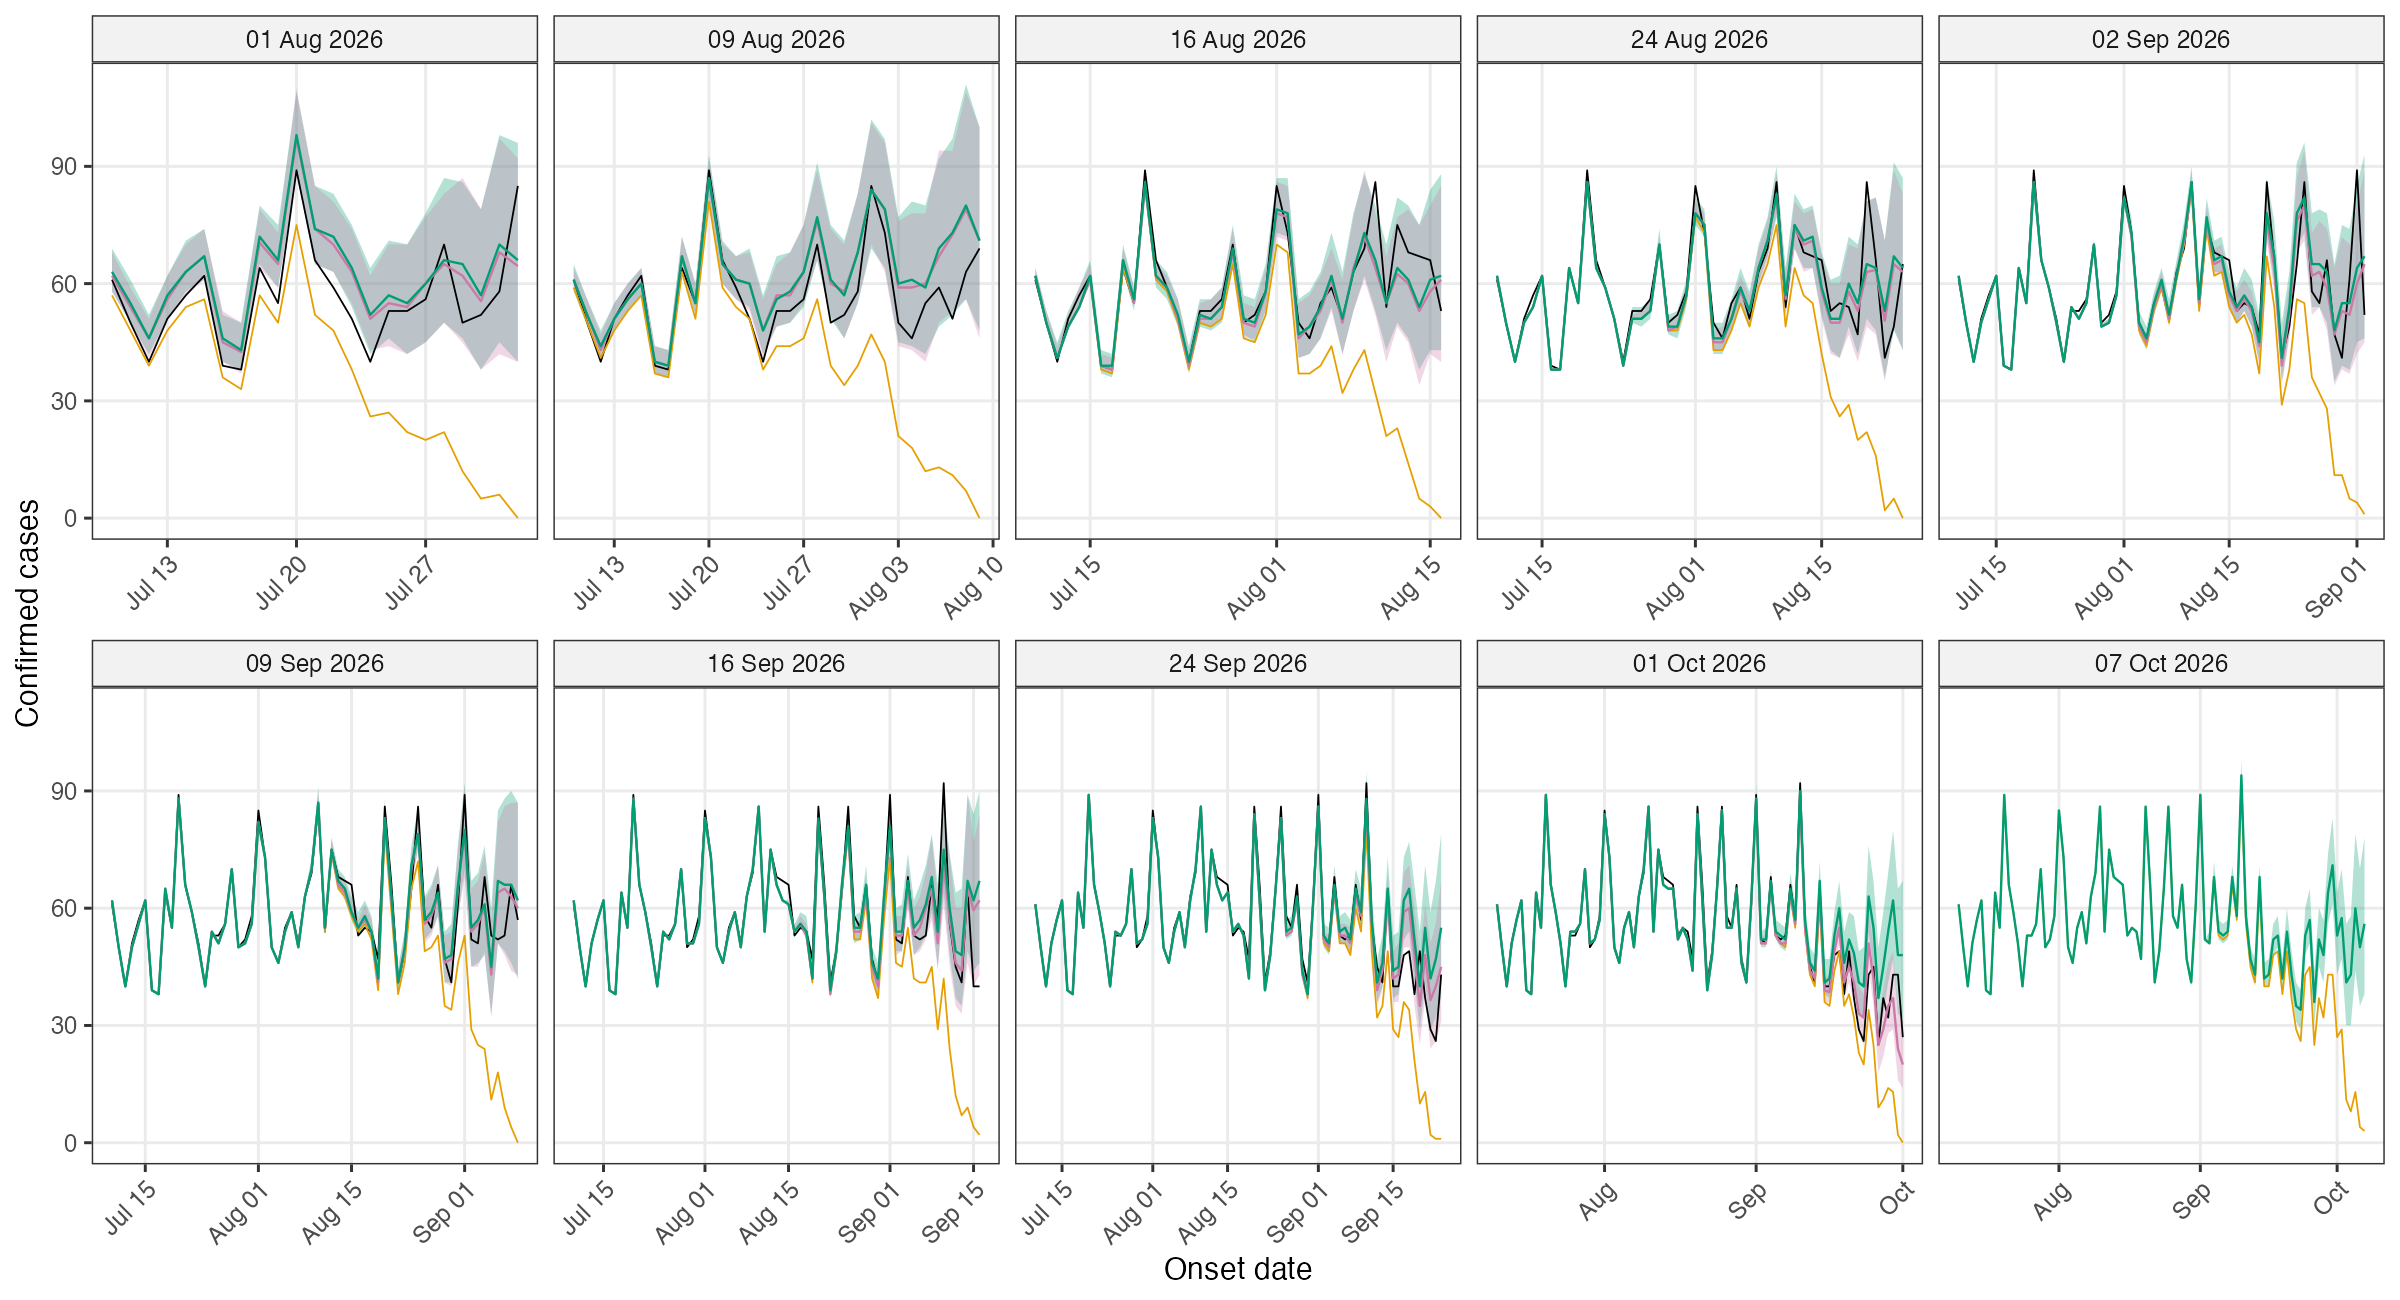
\includegraphics[height=0.8\textheight]{bvd_deaths_fits_cases.png}

{\small Panels: the date of each fit. Shading: 90\% interval of the projection.}
\end{frame}

% ---------------------------------------------------------------------------
\begin{frame}{Appendix: onset days first seen late}
The first report is that of 12 July, and already shows cases with onset
from April. The analysis starts at the onset day of 11 May.

\bigskip
\begin{itemize}
\item For these days the first report which includes them is treated as any
other, with nothing reported before it.
\item No change in the reporting delay of cases is allowed among them: they
say almost nothing about it.
\item Their recording delay is that of the first onset days whose early
reports are seen (to 18 July), so the deaths still being added months
later are left to the tail.
\end{itemize}
\end{frame}

% ---------------------------------------------------------------------------
\begin{frame}{Appendix: the report of 6 September}
This report corrected the records of onset days before 28 June: 137 records
removed, 48 added, and some records changed from dead to alive. The model
of wrong records (few, removed one at a time) cannot follow counts across
it.

\bigskip
\begin{itemize}
\item For the corrected onset days, the reports made before 6 September are
left out, and that report is treated as their first.
\item Those days are 71 to 118 days old when first seen, so $\cfr_t$ is close
to the share shown as dead.
\item What is given up: those earlier reports showed their deaths being
recorded over many weeks.
\end{itemize}
\end{frame}

% ---------------------------------------------------------------------------
% The slides on the model of cases (docs/bvd_slides.tex)
\begin{frame}
\centering
\Large Appendix: the model of cases
\end{frame}

% ---------------------------------------------------------------------------
\begin{frame}{Cases: the counts keep changing}
\centering
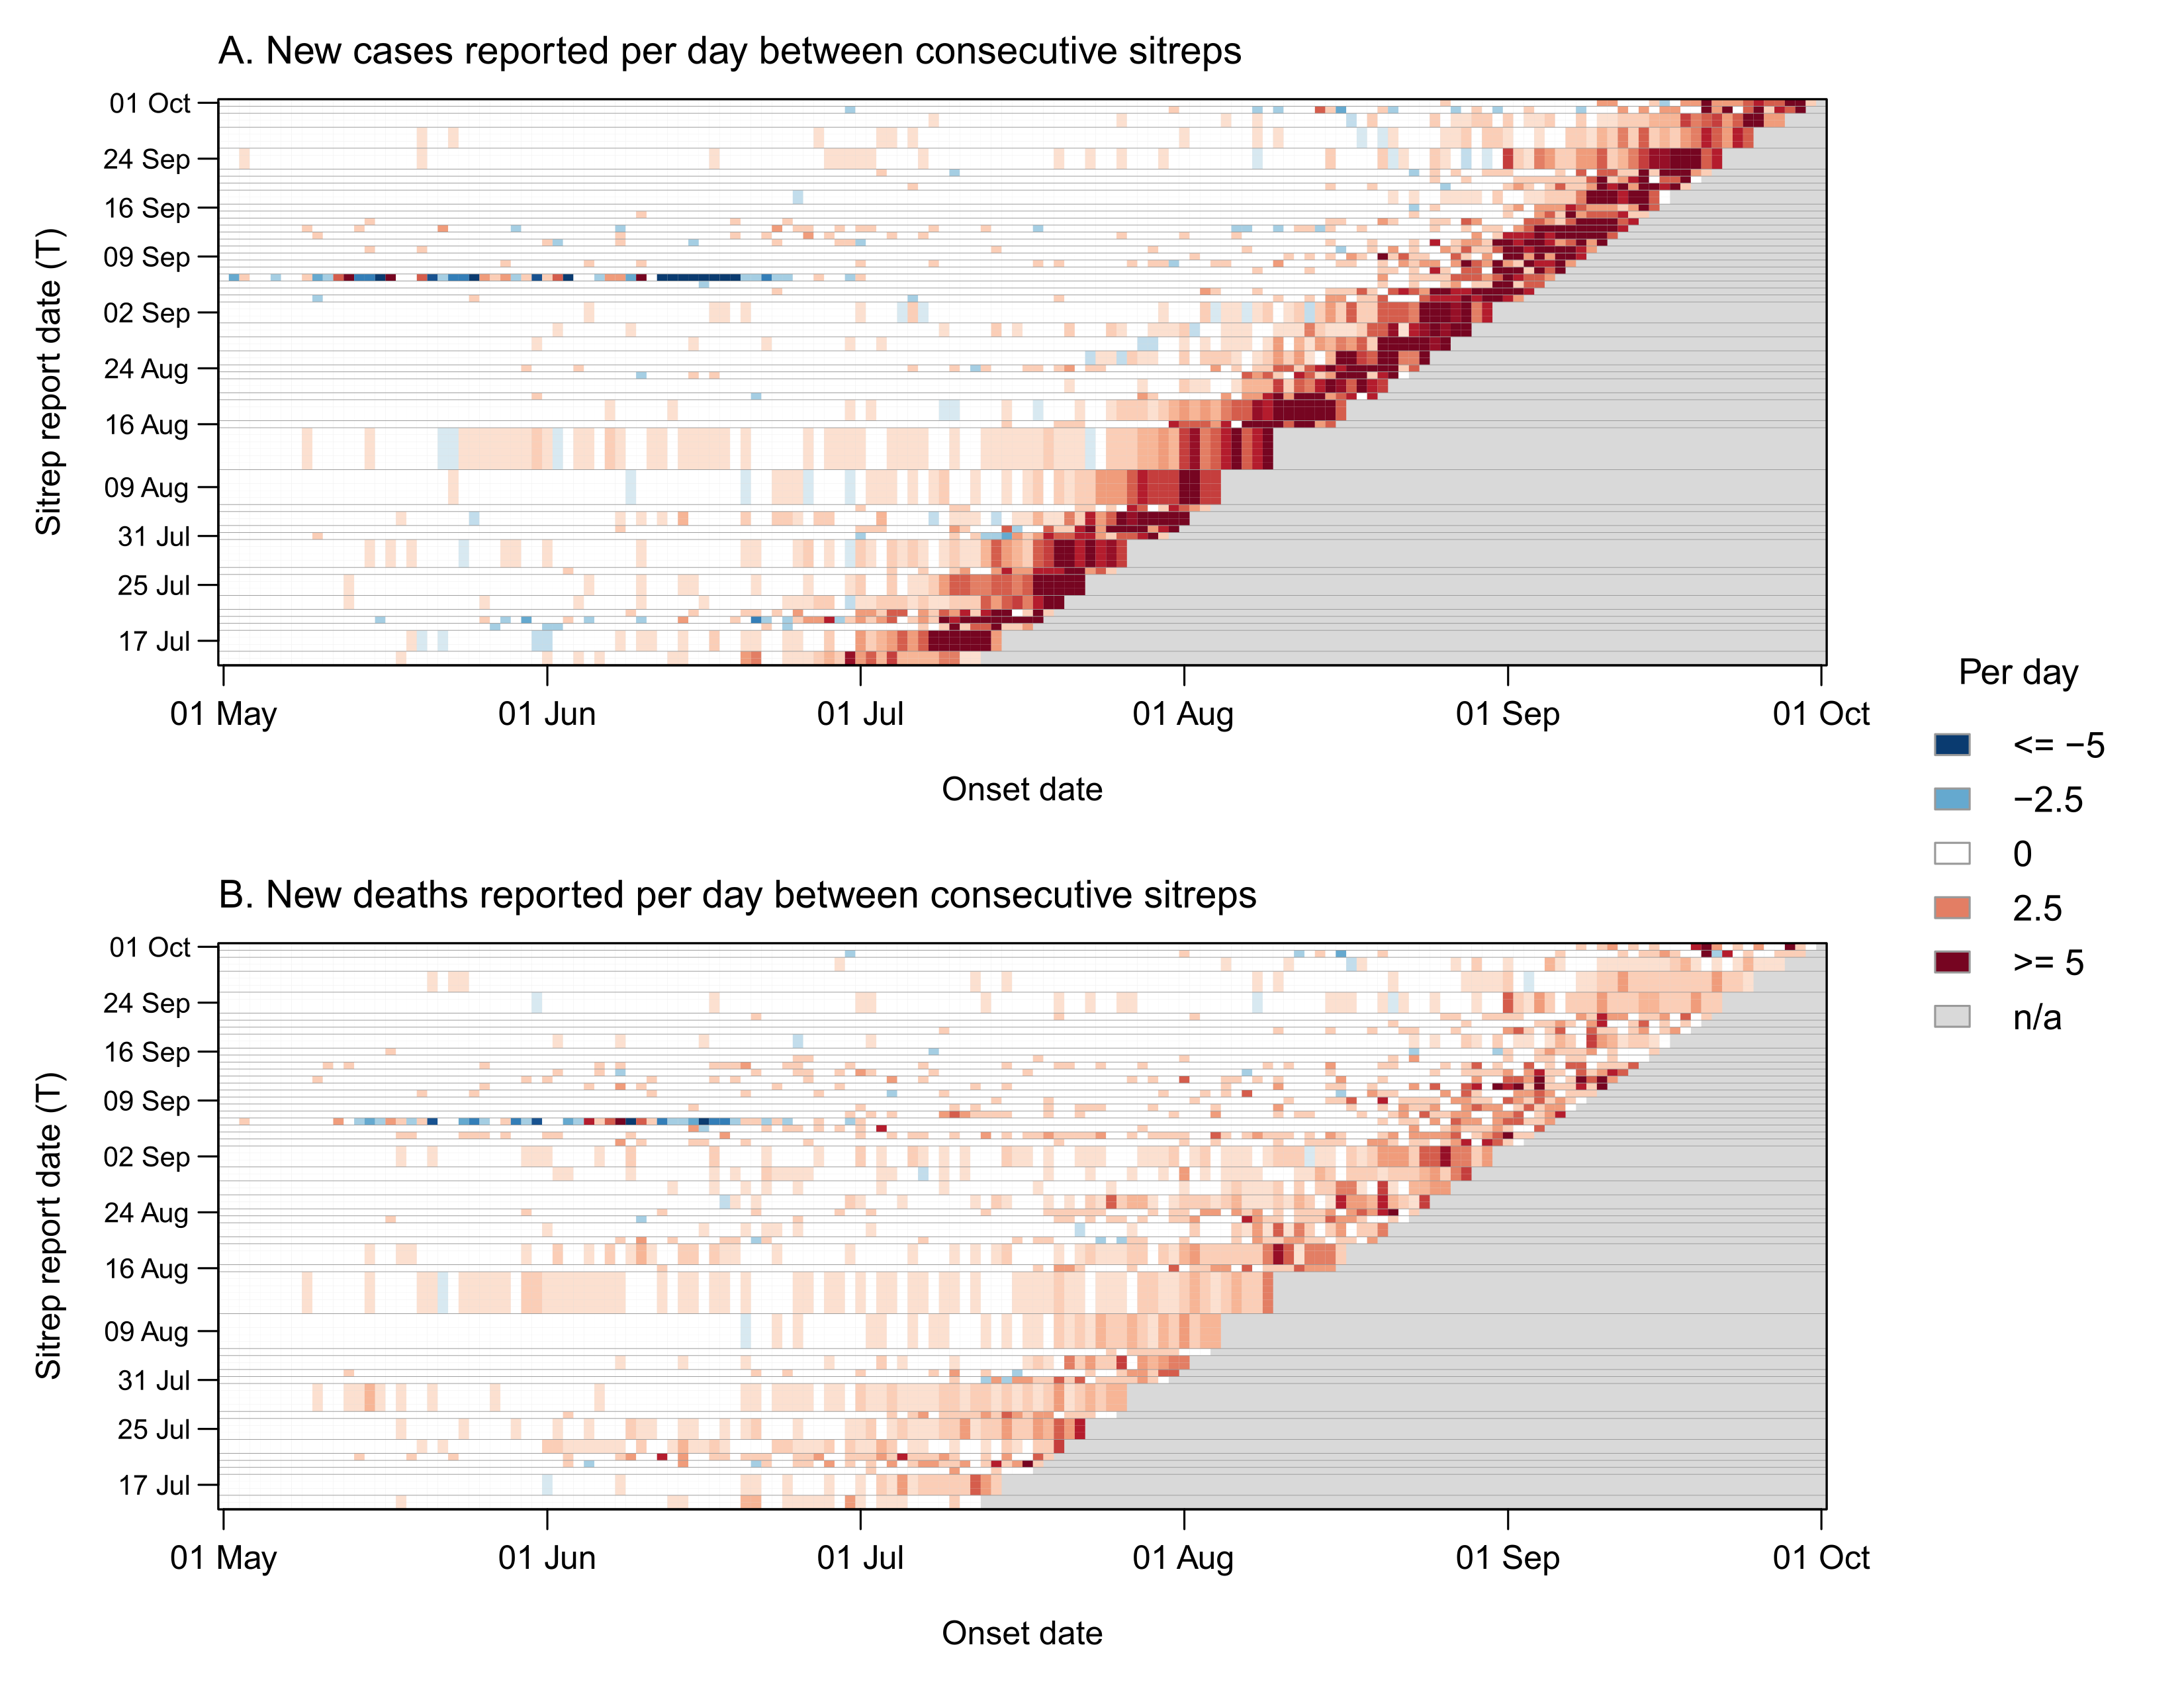
\includegraphics[height=0.74\textheight]{sitrep_increments.png}

\smallskip
{\small Counts for each onset date keep changing from one situation report to
the next: mostly added (red), sometimes removed (blue).}
\end{frame}

% ---------------------------------------------------------------------------
\begin{frame}{Cases: Approach}
Each report gives $C(t\given t')$: confirmed cases with onset on day $t$, as
known on day $t'$.

\bigskip
The true cases $I(t)$ are unknown. We model how they arise and how they come
to be reported:
\[
p\bigl(I, R, \theta \given C\bigr)\;\propto\;
\underbrace{p\bigl(C\given I,\theta\bigr)}_{\text{reporting}}\;
\underbrace{p\bigl(I\given R\bigr)}_{\text{transmission}}\;
p(R)\,p(\theta)
\]

\bigskip
\begin{itemize}
\item $R$: reproduction numbers $R_t$. $\theta$: parameters of reporting
(the delay distribution, effects of the day of the week, rates of misreporting).
\item $R_t$ and the delay can change at unknown times.
\end{itemize}

\bigskip
{\small Extends Bajaj, Thompson \& Lambert (2025).}
\end{frame}

% ---------------------------------------------------------------------------
\begin{frame}{Cases: Starting point: Bajaj, Thompson \& Lambert (2025)}
\textbf{Transmission.} True cases follow a renewal process, with $R_t$
constant within fixed windows:
\[
I(t)\sim\operatorname{Poisson}\Bigl(R_t\sum_{s\ge 1}\omega_s\,I(t-s)\Bigr)
\]

\textbf{Reporting.} Each case is reported after a random delay with survival
function $S_\theta$. Cases not yet reported at $t'$ are reported by $t''$
independently:
\[
C(t\given t'')-C(t\given t')\sim
\operatorname{binomial}\Bigl(I(t)-C(t\given t'),\
\frac{S_\theta(t'-t)-S_\theta(t''-t)}{S_\theta(t'-t)}\Bigr)
\]

\textbf{Inference.} Gibbs sampling over $I(t)$, $R_t$ and $\theta$:
\begin{itemize}
\item $I(t)$ from its discrete full conditional;
\item $R_t$ from a conjugate gamma;
\item $\theta$ by Metropolis.
\end{itemize}
\end{frame}

% ---------------------------------------------------------------------------
\begin{frame}{Cases: Changing some things...}
\centering
\renewcommand{\arraystretch}{1.5}
\begin{tabular}{p{0.44\textwidth}p{0.46\textwidth}}
\toprule
\textbf{Original model} & \textbf{Here} \\
\midrule
Counts can only rise, and never exceed $I(t)$ & Records can be added in error and later removed \\
Reporting depends only on the delay & Reports differ by day of the week \\
One delay distribution, or periods fixed in advance & The delay can change at unknown times \\
$R_t$ constant within fixed windows & $R_t$ can change at unknown times \\
Series starts with the outbreak & Earlier cases enter as known \\
\bottomrule
\end{tabular}
\end{frame}

% ---------------------------------------------------------------------------
\begin{frame}{Cases: The data}
\centering
\renewcommand{\arraystretch}{1.25}
\resultsinput{bvd_data.tex}

\medskip
\begin{minipage}{0.8\textwidth}
\small $^{*}$Every report gives a count for every onset day so far. For each
onset day, we compare its count in each report with its count in the report
before: for example, cases with onset on 1 August numbered 10 in the report
of 3 August and 13 in the report of 4 August, so that count went up. Over all
onset days and all pairs of consecutive reports there are this many
comparisons.
\end{minipage}
\end{frame}

% ---------------------------------------------------------------------------
\begin{frame}{Cases: Transmission}
\[
I(t)\sim\operatorname{NB}\bigl(R_t\,\Lambda_t,\ \kappa\bigr),\qquad
\Lambda_t=\sum_{s=1}^{40}\omega_s\,I(t-s)
\]

\bigskip
\begin{itemize}
\item $\omega_s$: discretised gamma serial interval (mean 15.3, sd 9.3 days;
Zaire ebolavirus).
\item Cases with onset \bvdDateBeforeFirst{} to \bvdDateBeforeLast{} (the 40
days before the first report) are not modelled: their counts in the report of
\bvdDateLatest{} enter $\Lambda_t$ as fixed values.
\item $R_t$ is piecewise constant (next slide).
\end{itemize}
\end{frame}

% ---------------------------------------------------------------------------
\begin{frame}{Cases: Piecewise-constant parameters, with changes at unknown times}
Used for $R_t$ and for the delay parameters $(\mu,\sigma)$. Onset days
$1,\dots,T$ are split into segments; the parameter is constant within each.

\medskip
\[
p(\tau_1,\dots,\tau_K\given p)\propto p^{K}(1-p)^{T-1-K},\qquad
p\sim\operatorname{beta}(1,T)
\]

\begin{columns}[c]
\begin{column}{0.5\textwidth}
\begin{itemize}
\item $\tau_1<\dots<\tau_K$: the days on which a new segment starts (the
change points).
\item Each day starts a new segment with probability $p$ (Barry \& Hartigan
1992).
\item Minimum segment: 7 days ($R_t$), 14 days (delay).
\item The number of changes $K$ is inferred.
\end{itemize}
\end{column}
\begin{column}{0.45\textwidth}
\centering
Implied prior for $R_t$

\smallskip
\begin{tabular}{lcccc}
\toprule
$K$ & 0 & 1 & 2 & $\ge 3$ \\
\midrule
Probability & 0.61 & 0.26 & 0.09 & 0.04 \\
\bottomrule
\end{tabular}
\end{column}
\end{columns}
\end{frame}

% ---------------------------------------------------------------------------
\begin{frame}{Cases: Reporting delays}
A case with onset on day $t$ is reported after a gamma$(\mu,\sigma)$ delay.
$S_\theta(t\given k)$: probability it is still unreported at the end of day
$k$. Its hazard of being reported on day $k$:
\[
h_\theta(t,k)=\log S_\theta(t\given k-1)-\log S_\theta(t\given k)
\]

\smallskip
Reports differ by day of the week, so each day's hazard is multiplied by
$m_k=\psi_w$, where $w$ is the weekday of the next report:
\[
S^{*}_\theta(t\given t')=S_\theta(t\given t)\,
\exp\Bigl\{-\sum_{k=t+1}^{t'}m_k\,h_\theta(t,k)\Bigr\}
\]

{\small $S_\theta(t\given t)$: probability a case is not reported on its day
of onset (about 0.99 here).}

\smallskip
A case unreported at report $t_{j-1}$ appears in report $t_j$ with
probability
$\displaystyle p(t\given t_j)=1-\frac{S^{*}_\theta(t\given t_j)}{S^{*}_\theta(t\given t_{j-1})}$.
\end{frame}

% ---------------------------------------------------------------------------
\begin{frame}{Cases: Misreporting: the idea}
Counts sometimes fall, so some records in them must be wrong: duplicates,
cases later reclassified, wrong onset dates.

\bigskip
Split the count for onset day $t$ in the report of day $t_j$ into two parts,
neither observed:
\[
C(t\given t_j)=\underbrace{C^{G}(t\given t_j)}_{\substack{\text{genuine cases}\\\text{reported so far}}}
+\underbrace{E(t\given t_j)}_{\substack{\text{wrong records}\\\text{currently in the count}}}
\]

\medskip
\begin{itemize}
\item \textbf{Errors are made when cases are being reported.} Each genuine
report brings, on average, $\eta$ wrong records with it.
\item \textbf{Errors are found later.} Each wrong record is removed with
probability $\rho$ each day.
\end{itemize}
\end{frame}

% ---------------------------------------------------------------------------
\begin{frame}{Cases: Misreporting: the model}
Between reports $t_{j-1}$ and $t_j$, for onset day $t$:

\medskip
\begin{align*}
\text{genuine cases, newly reported}\quad & \Delta C^{G}(t\given t_j)\sim\operatorname{binomial}\bigl(I(t)-C^{G}(t\given t_{j-1}),\ p(t\given t_j)\bigr)\\[3pt]
\text{wrong records added}\quad & n(t\given t_j)\sim\operatorname{Poisson}\bigl(\eta\times
\underbrace{I(t)\,[S^{*}_\theta(t\given t_{j-1})-S^{*}_\theta(t\given t_j)]}_{\text{expected genuine reports}}\bigr)\\[3pt]
\text{wrong records removed}\quad & e(t\given t_j)\sim\operatorname{binomial}\bigl(E(t\given t_{j-1}),\ 1-(1-\rho)^{t_j-t_{j-1}}\bigr)
\end{align*}
\[
C^{G}(t\given t_j)=C^{G}(t\given t_{j-1})+\Delta C^{G}(t\given t_j),\qquad E(t\given t_j)=E(t\given t_{j-1})+n(t\given t_j)-e(t\given t_j)
\]

\smallskip
\small
\begin{itemize}
\item Wrong records are added in proportion to reporting activity: many when
an onset day is being reported, almost none once it is complete.
\item A wrong record survives each day with probability $1-\rho$, so
$1-(1-\rho)^{t_j-t_{j-1}}$ is the probability it is removed at some point in
the $t_j-t_{j-1}$ days between the two reports.
\item Only $C=C^{G}+E$ is observed. We marginalise over $E$ exactly by a forward
recursion over reports, truncated at $E\le\bvdErroneousMax$ (one more than
the largest fall seen in a count).
\end{itemize}
\end{frame}

% ---------------------------------------------------------------------------
\begin{frame}{Cases: Fitting}
Metropolis within Gibbs.

\bigskip
\begin{itemize}
\item $I(t)$: drawn from its discrete full conditional.
\item $R_t$ segments: drawn exactly, with segment values integrated out.
\item Delay segments: split, merge and shift moves.
\item $\kappa$, $\psi_w$, $\eta$, $\rho$: random-walk Metropolis.
\end{itemize}
\end{frame}

% ---------------------------------------------------------------------------
\begin{frame}{Cases: Past performance on cases}
\centering
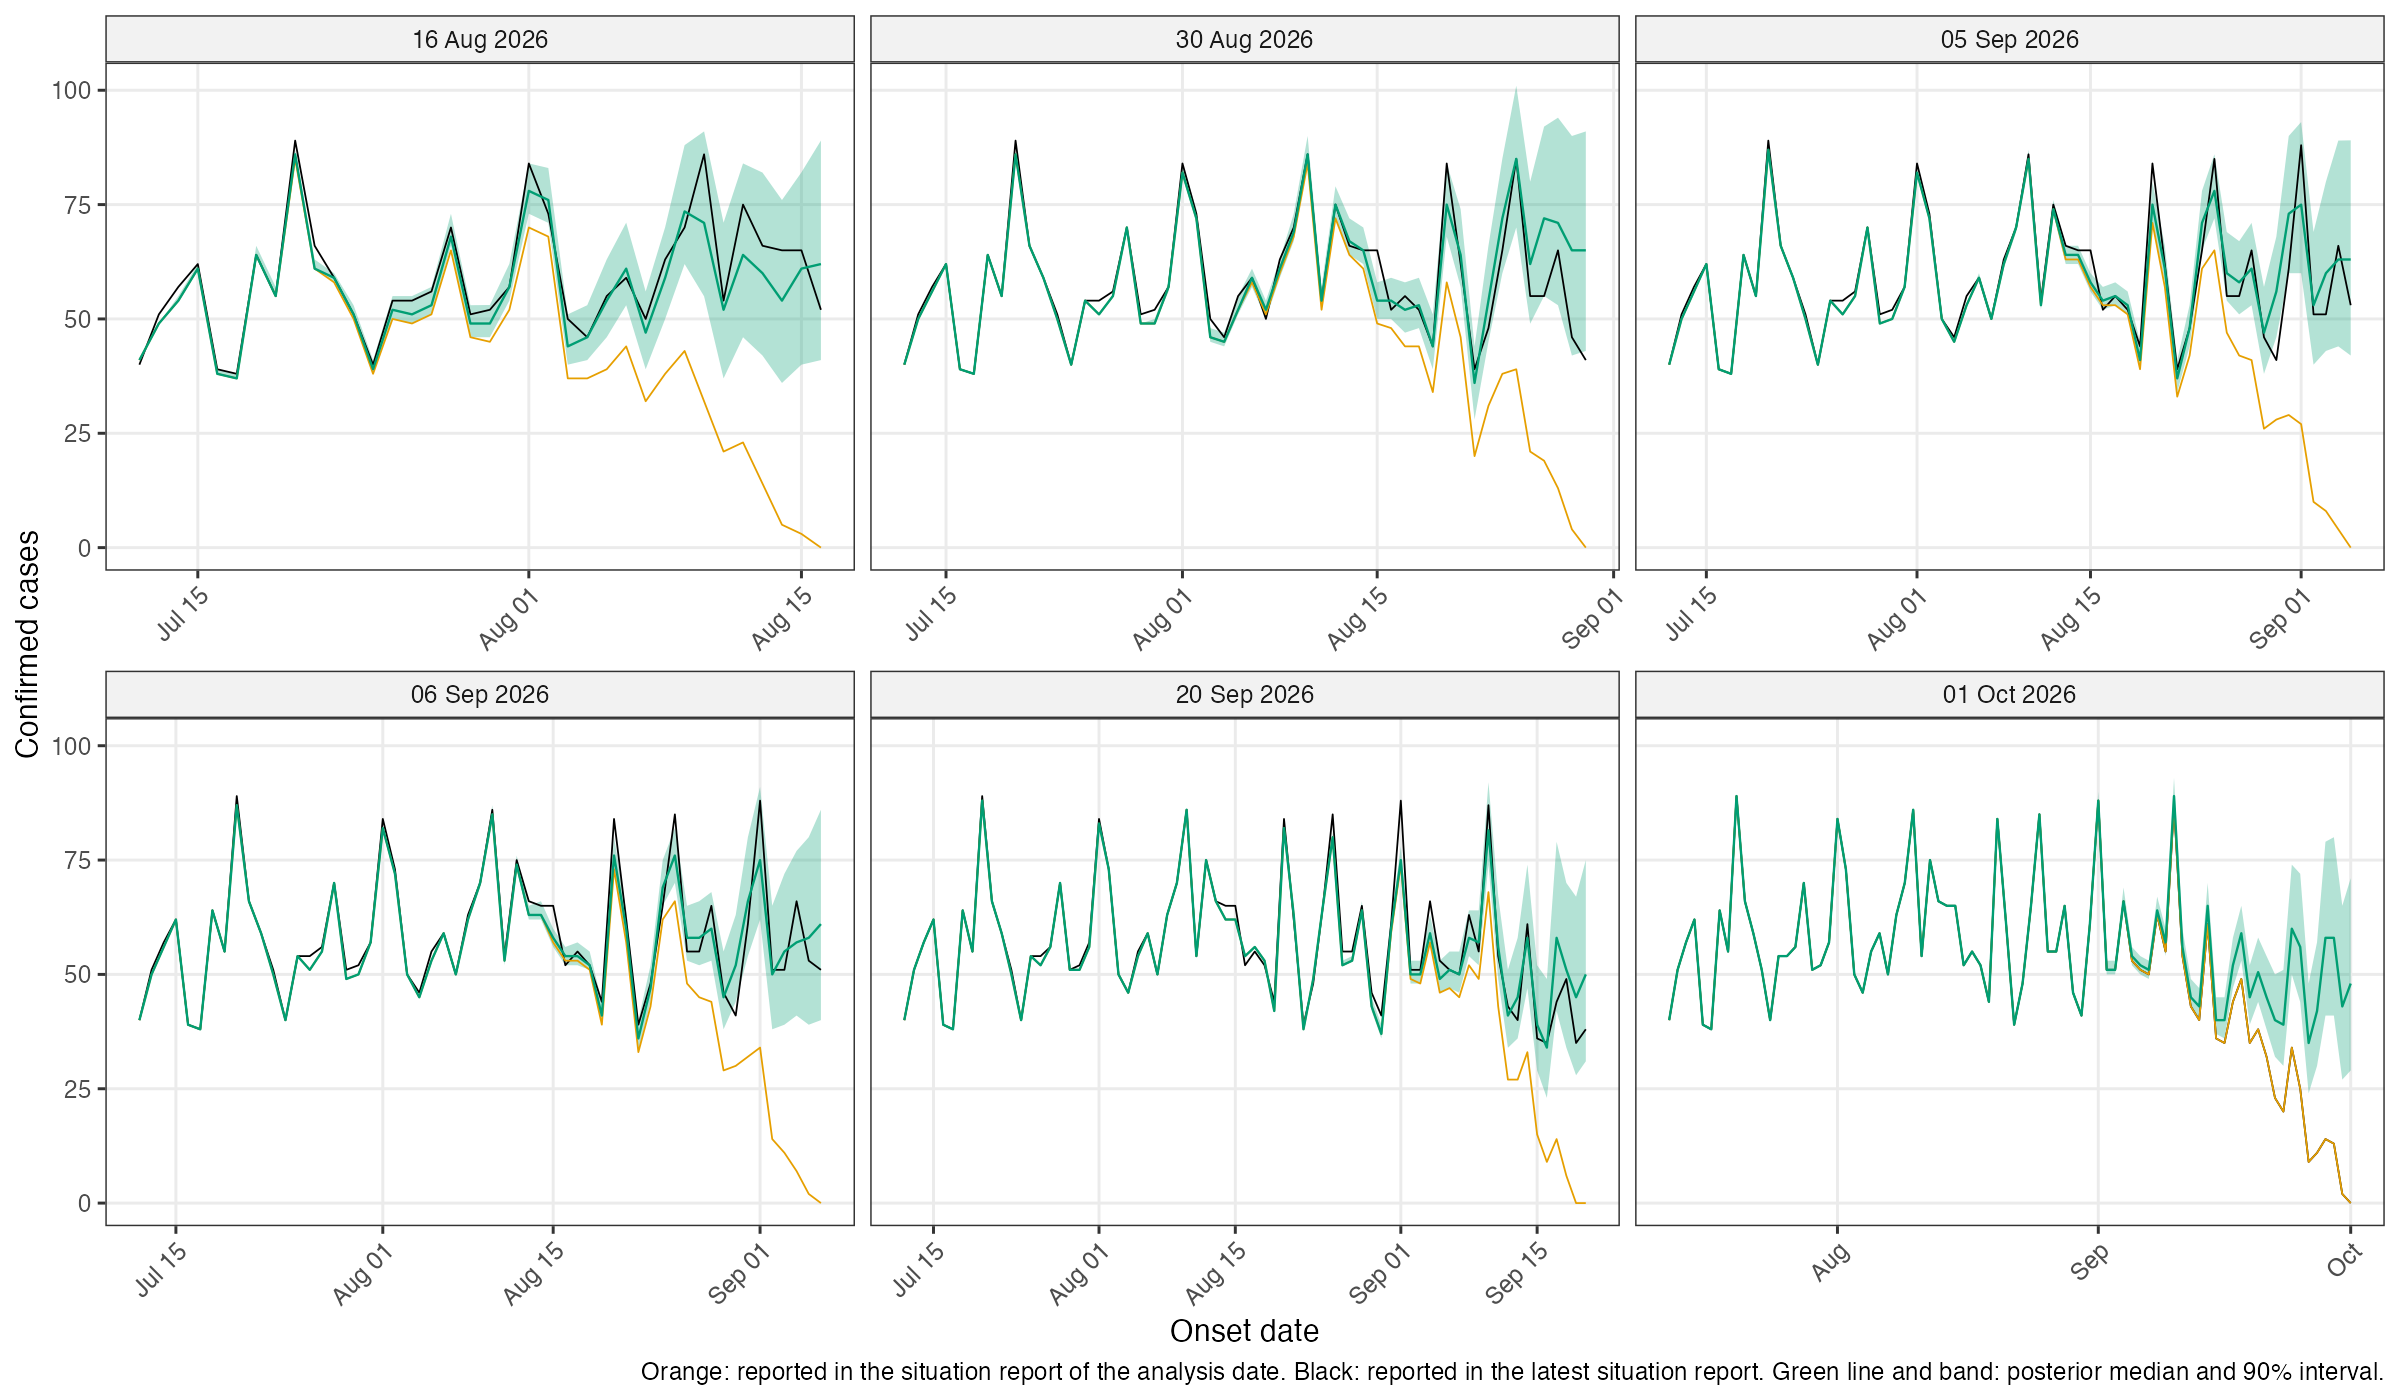
\includegraphics[height=0.78\textheight]{bvd_changepoint_cases.png}

{\small Orange: reported at the analysis date. Black: reported on
\bvdDateLatest. Green: posterior median and 90\% interval.}
\end{frame}

% ---------------------------------------------------------------------------
\begin{frame}{Cases: Results as of 1 October 2026}
\begin{columns}[c]
\begin{column}{0.68\textwidth}
\centering
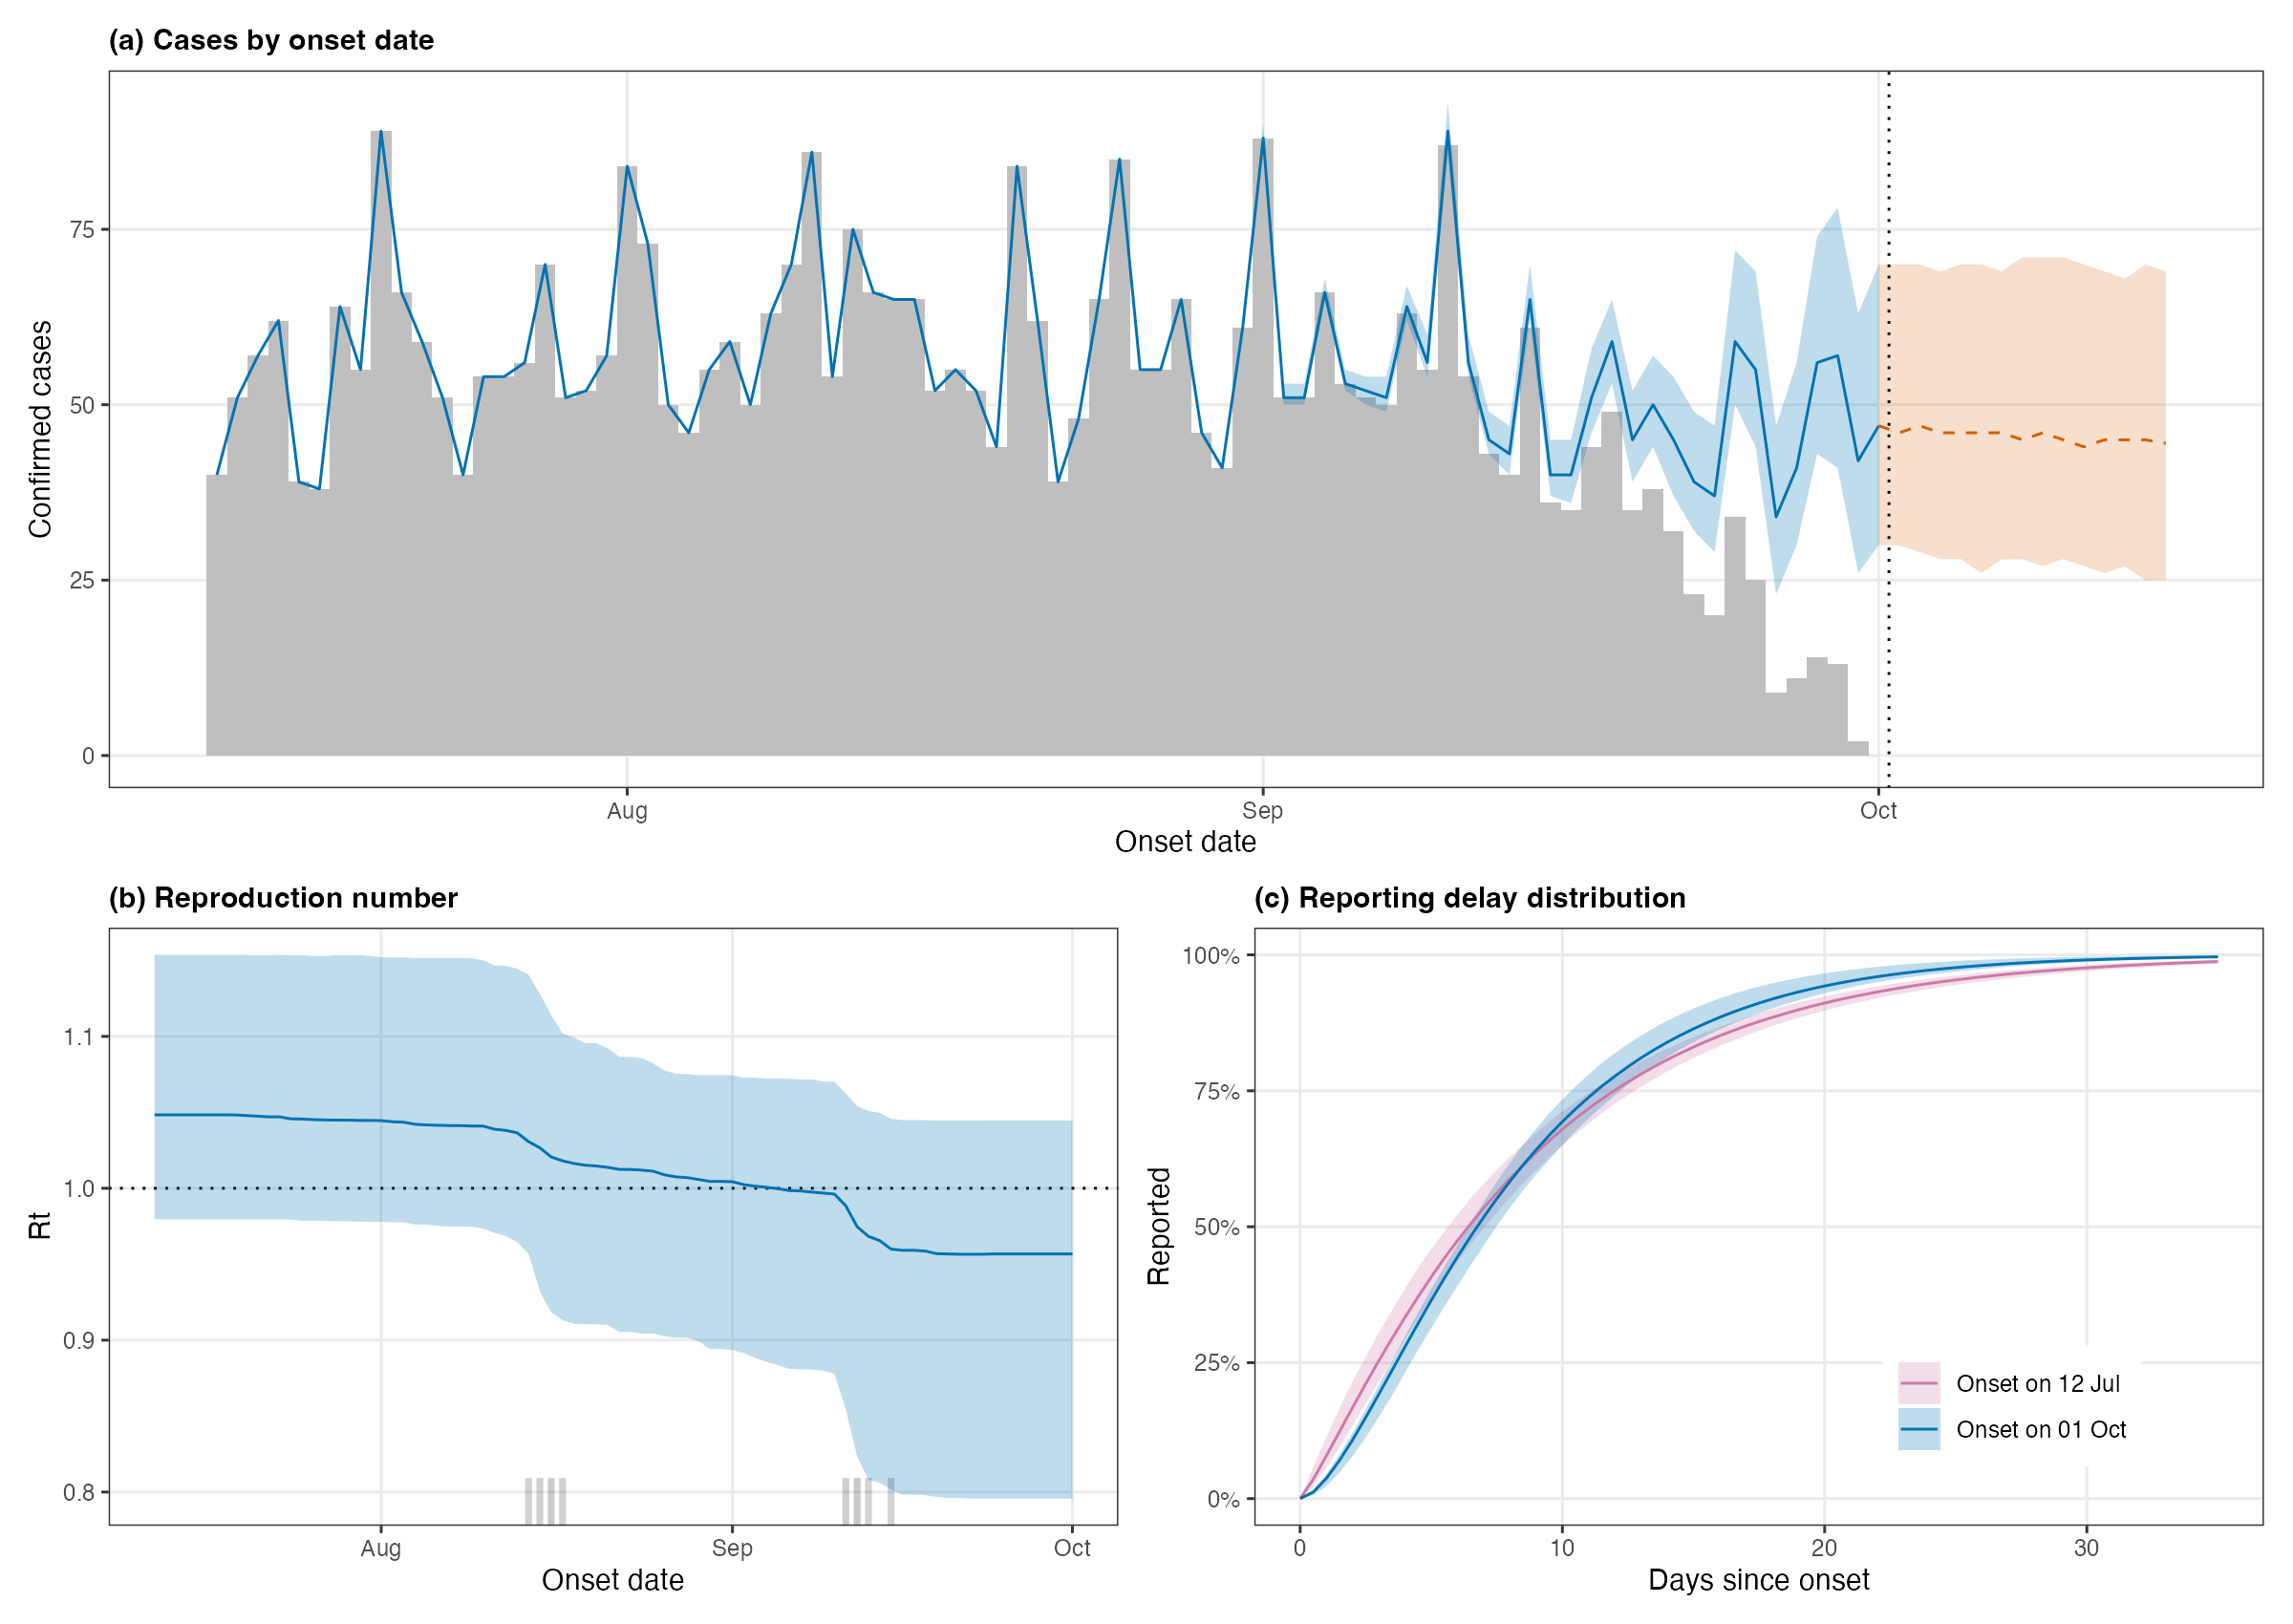
\includegraphics[width=\textwidth]{bvd_changepoint_main.png}
\end{column}
\begin{column}{0.3\textwidth}
{\small Grey: reported. Blue: estimated. Orange: projected at the latest $R_t$.}

\bigskip
$R_t$ now: \bvdRt.

\bigskip
Probability $R_t$ has not changed since \bvdDateFirst: \bvdRtNoChange{}
(the share of posterior draws with $K=0$; prior 0.61).

\bigskip
Delay now: mean \bvdDelayMean{} days, sd \bvdDelaySd{} days.
\end{column}
\end{columns}
\end{frame}

% ---------------------------------------------------------------------------
\begin{frame}{Cases: recovering changes from simulated data}
\centering
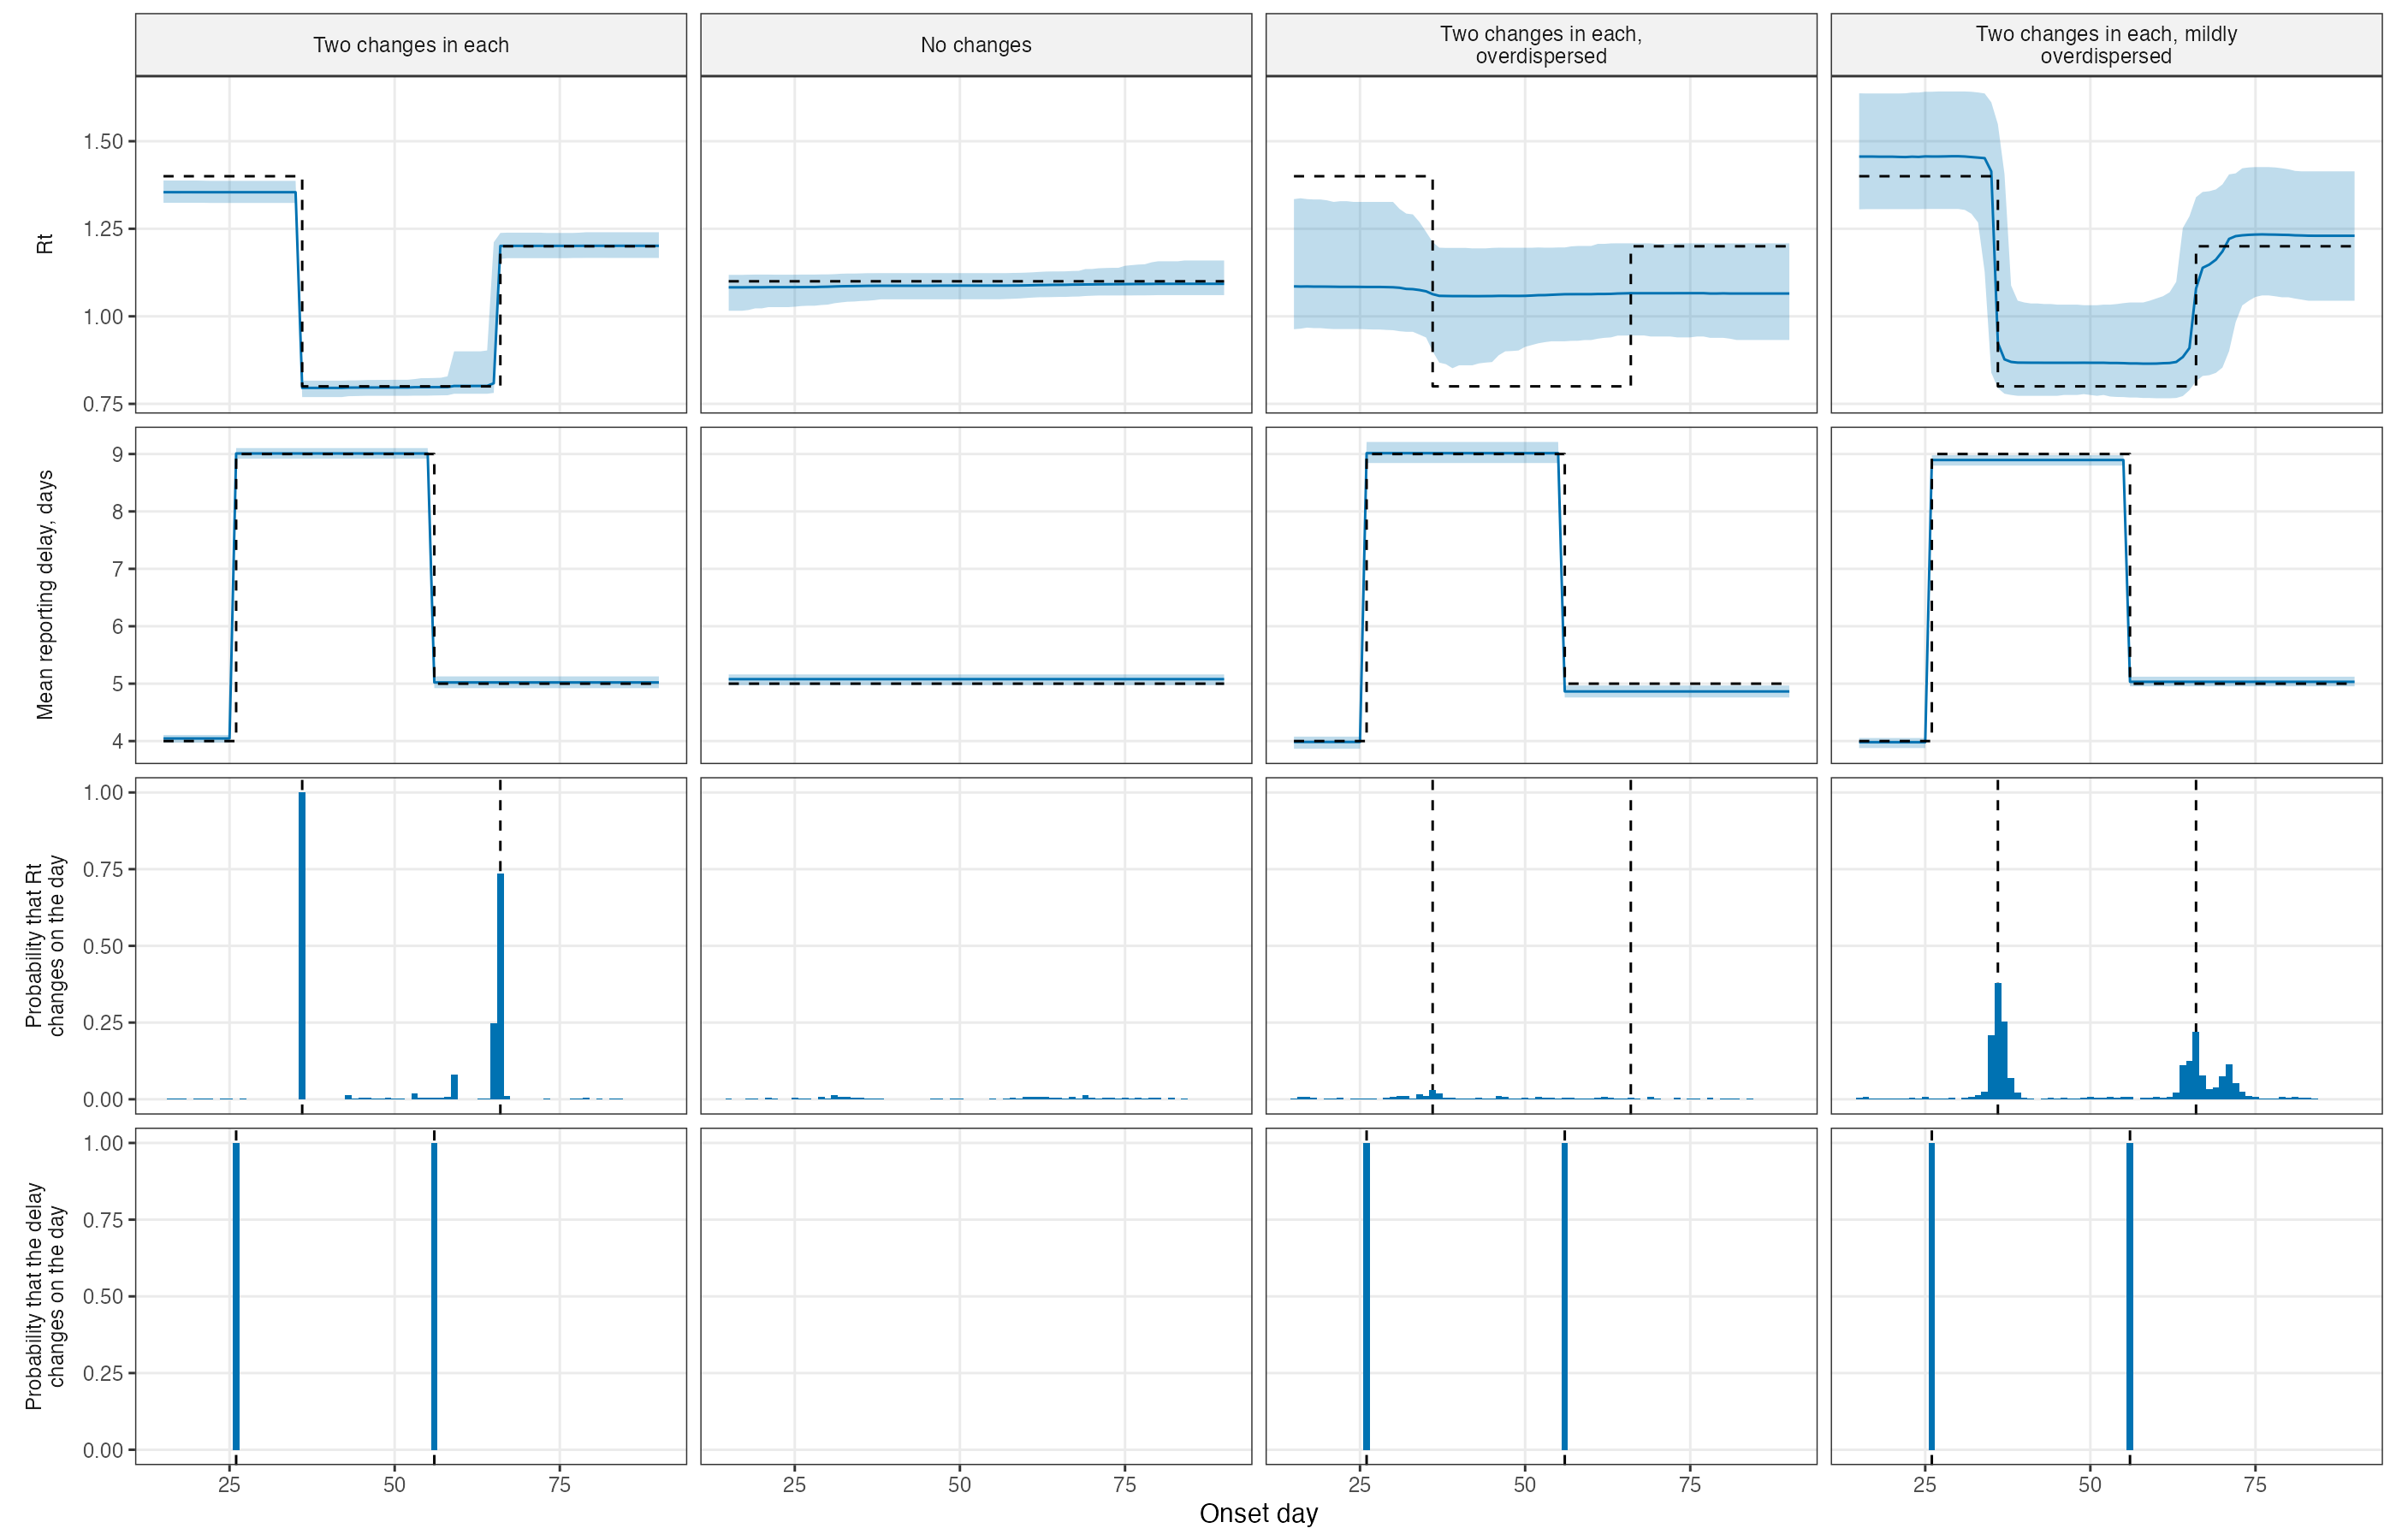
\includegraphics[height=0.82\textheight]{changepoint_demonstrations.png}
\end{frame}

% ---------------------------------------------------------------------------
\begin{frame}{Cases: further estimates as of 1 October 2026}
\centering
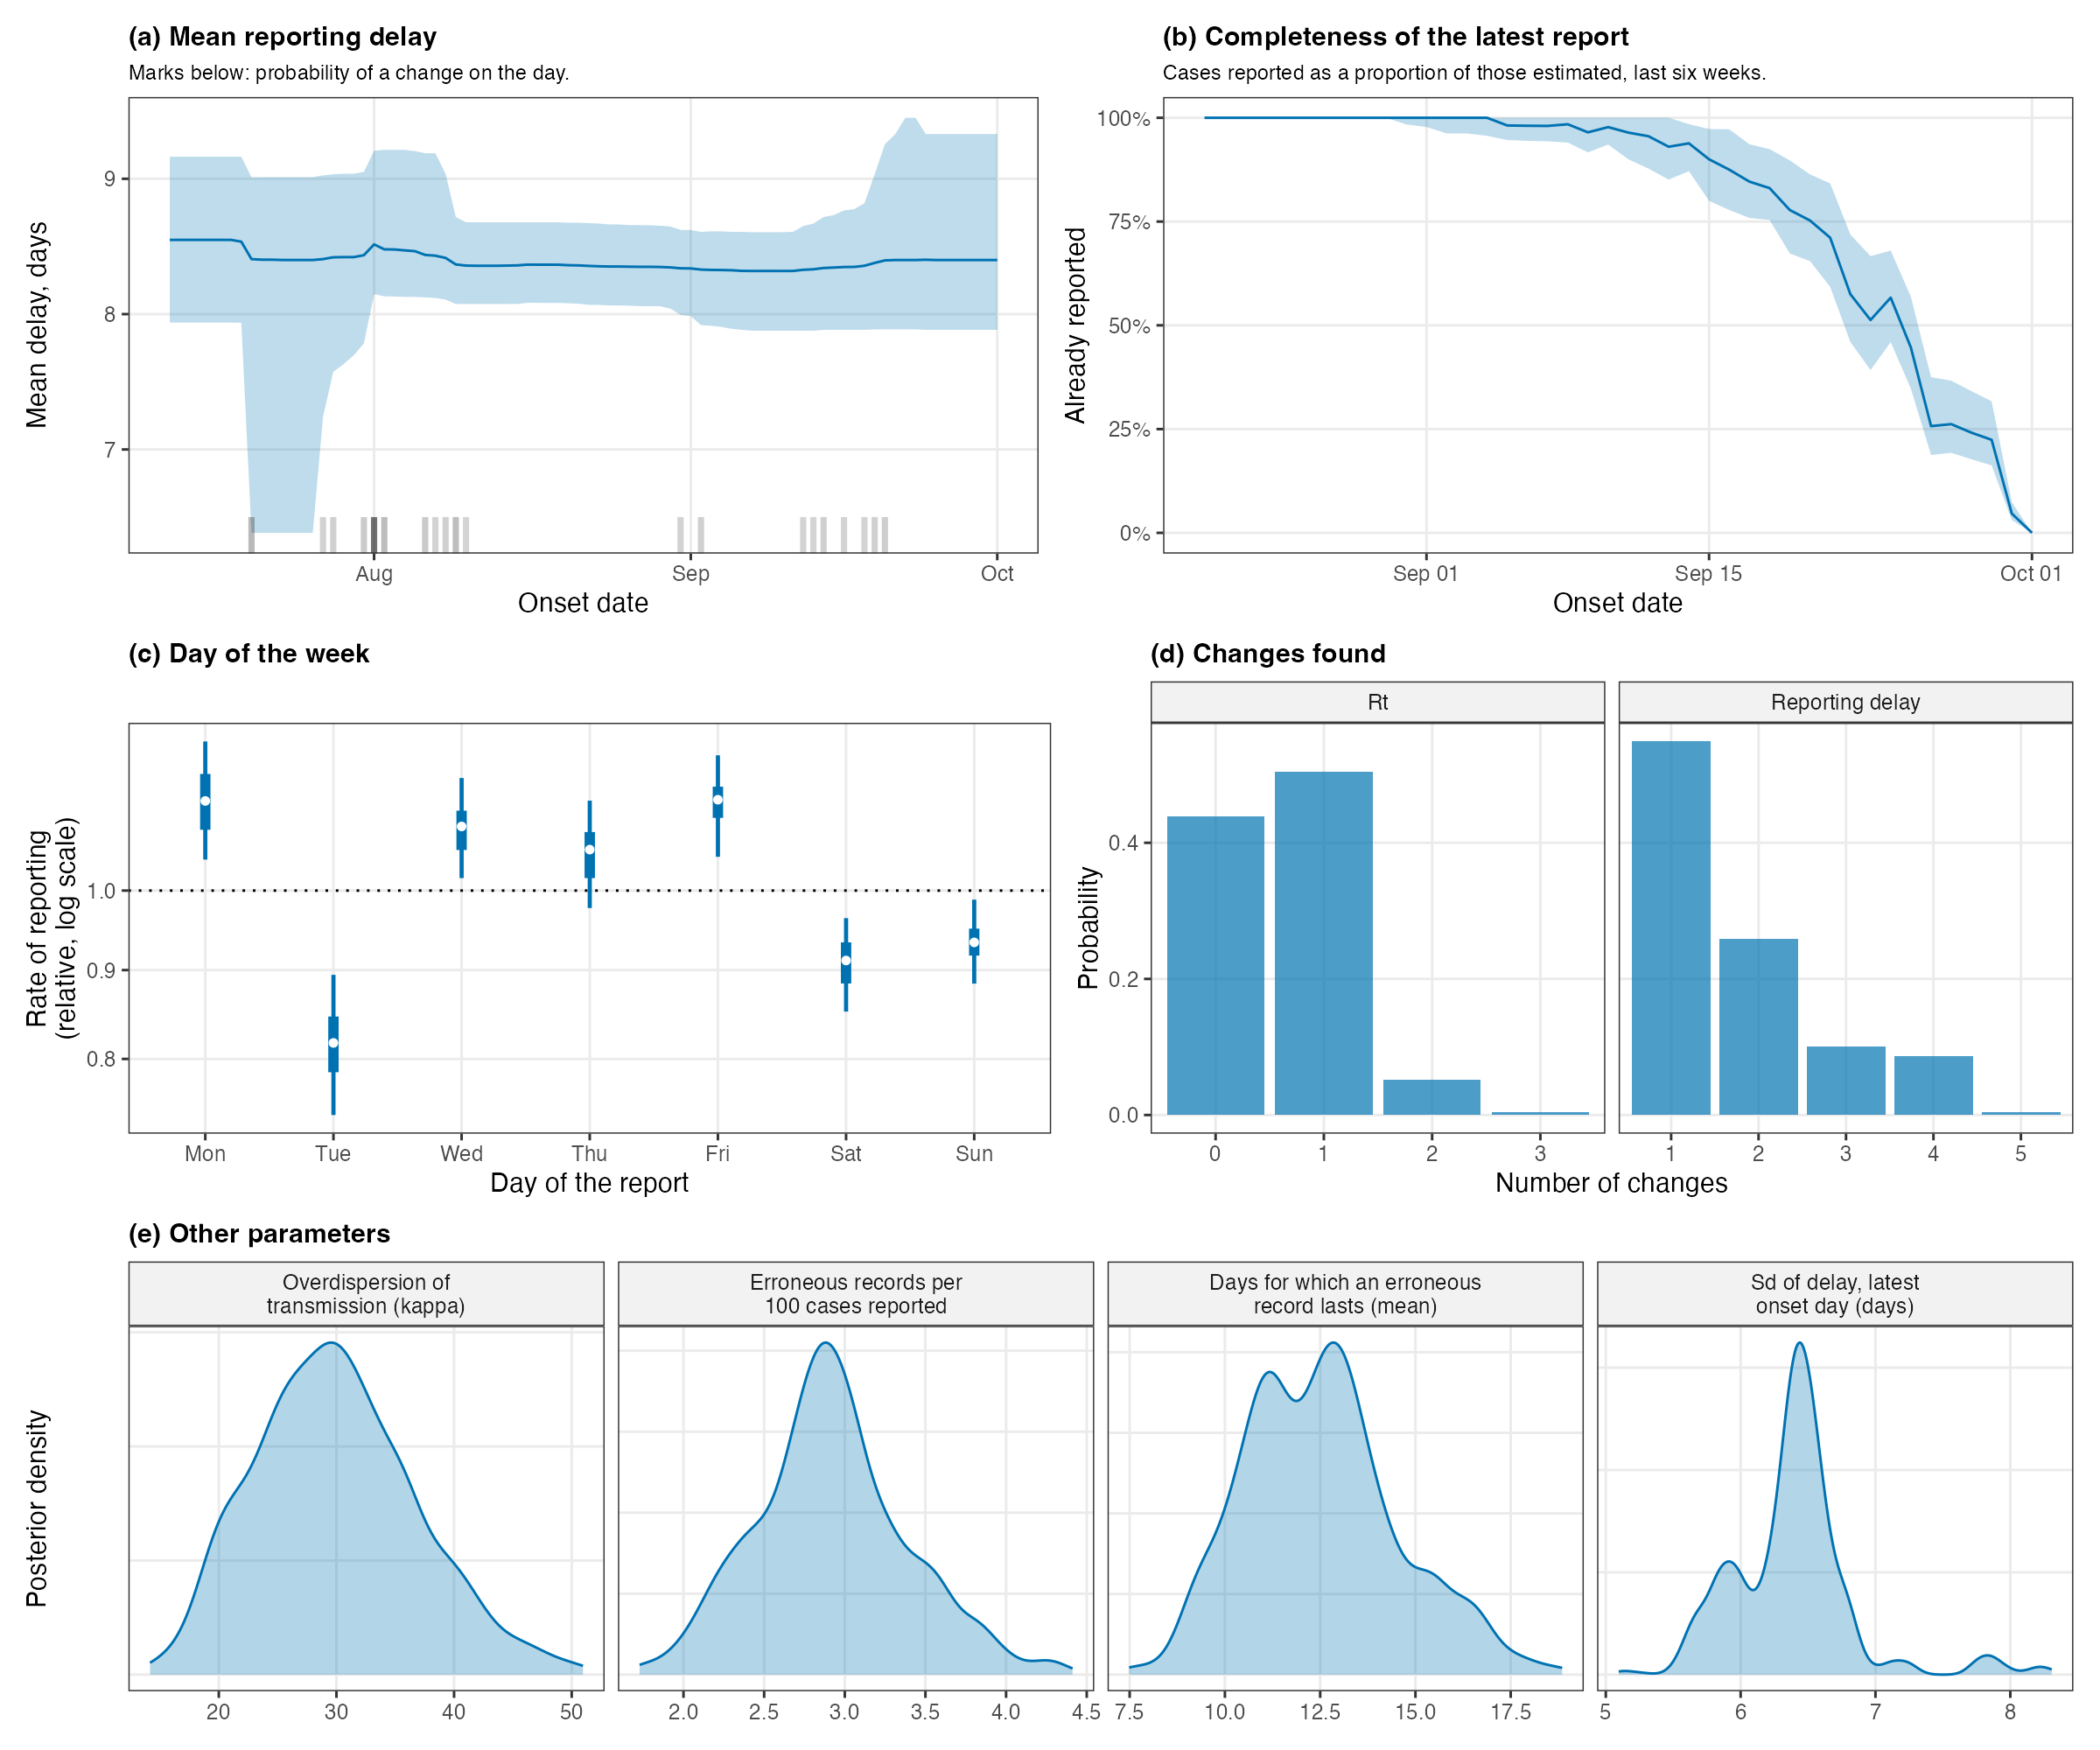
\includegraphics[height=0.82\textheight]{bvd_changepoint_parameters.png}
\end{frame}

% ---------------------------------------------------------------------------
\begin{frame}{Cases: parameter estimates as of 1 October 2026}
\centering
\renewcommand{\arraystretch}{1.1}
\resultsinput{bvd_parameters.tex}
\end{frame}

\end{document}
